\documentclass[a4paper,12pt,twoside]{scrreprt}
% Autor der Vorlage: Klaus Rheinberger, FH Vorarlberg, 2017-02-20

%% Pakete
% Dokumenteneigenschaften
\usepackage[ngerman]{babel}                 % Deutsche Sprachanpassungen
\usepackage[T1]{fontenc}                    % Silbentrennung bei Sonderzeichen
\usepackage[bindingoffset=8mm]{geometry}    % Bindeverlust von 8mm einbeziehen
\usepackage{minted}                         % Code Highlighting/Import
\usepackage{setspace}                       % Zeilenabstand

% Bilder & PDFs
\usepackage{graphicx} % Bilder einbinden
\usepackage{wrapfig}  % Bilder positionieren
\usepackage{pdfpages} % PDFs einbetten

% Zitate & Verweise, Sonstiges
\usepackage[nohyperlinks]{acronym}  % Abkürzungsverzeichnis
\usepackage{caption}                % Abbildungslegenden
\usepackage{csquotes}               % Anführungszeichen und Zitieren
\usepackage[]{hyperref}             % Links
\usepackage[
    style=ieee,
    citestyle=ieee,
    backend=biber
]{biblatex}                         % Literaturverweise
\usepackage{xcolor}                 % Farbige Hervorhebungen

%% Einstellungen
\addbibresource{references.bib}
\onehalfspacing
\setcounter{secnumdepth}{4} % Nummerierungstiefe
\setcounter{tocdepth}{3}    % Gliederungstiefe Inhaltsverzeichnis

%% Dokument
\begin{document}

% Titelblatt
\pagenumbering{roman}

\begin{titlepage}
    \begin{flushright}
    
\includegraphics[width=0.4\linewidth]{images/FHV_FHV-Logo.png}
    \end{flushright}
    \vspace{1cm}

    \begin{flushleft}
    \section*{Praxisnahe Anwendung der User-Centered Design Prinzipien}
    \subsection*{Neuentwicklung des Ethikantrag-Tools der Forschungsethik-Kommission der Fachhochschule Vorarlberg}
    \vspace{1cm}

    Masterarbeit\\
    zur Erlangung des akademischen Grades
    \vspace{0.5cm}

    \textbf{Master of Science in Engineering (MSc)}

    \vspace{1cm}
    Fachhochschule Vorarlberg\newline
    Informatik Master

    \vspace{0.5cm}

    Betreut von\newline
    Karin Trommelschläger, MSc

    \vspace{0.5cm}

    Vorgelegt von\newline
    Dominic Luidold, BSc\newline
    Dornbirn, [Monat Jahr]
    \end{flushleft}
\end{titlepage}

% Widmung
\newpage
\section*{Widmung}
\label{sec:widmung}

\colorbox{yellow}{TODO - Widmung}

% Abstract [DE]
\newpage
\section*{Kurzreferat}
\label{sec:abstract-de}

\subsection*{Titel [DE]}

\colorbox{yellow}{TODO - Kurzreferat}

% Abstract [EN]
\newpage
\section*{Abstract}
\label{sec:abstract-en}

\subsection*{Titel [EN]}

\colorbox{yellow}{TODO - Abstract}

% Inhaltsverzeichnis
\cleardoublepage
\tableofcontents

% Abbildungsverzeichnis
\clearpage
\phantomsection
\addcontentsline{toc}{chapter}{Abbildungsverzeichnis}
\listoffigures

% Abkürzungsverzeichnis
\clearpage
\phantomsection
\addcontentsline{toc}{chapter}{Abkürzungsverzeichnis}
\chapter*{Abkürzungsverzeichnis}

\begin{acronym}
    \acro{ecs}[ECS]{Ethic Commission System}
    \acro{fek}[FE-K]{Forschungsethik-Kommission}
    \acro{fhv}[FHV]{Fachhochschule Vorarlberg}
    \acro{föe}[FÖE]{Forum Österreichischer Ethikkommissionen}
    \acro{ieb}[IEB]{Institutionelle Ethikboard der Fachhochschule Gesundheitsberufe OÖ}
    \acro{poc}[PoC]{Proof of Concept}
    \acro{ux}[UX]{User Experience}
\end{acronym}

% Inhalt
\cleardoublepage
\pagenumbering{arabic}

\chapter{Einleitung}
\label{chap:einleitung}

Die vorliegende Masterarbeit beschäftigt sich mit dem Erstellen und Einreichen von Ethikanträgen, die bei der \ac{fek} der \ac{fhv}\footnote{\href{https://www.fhv.at/forschung/forschungsethik-kommission/}{Forschungsethik-Kommission: Analyse von Forschungstätigkeiten und deren ethischer Grundsatzfragen (\url{https://www.fhv.at/forschung/forschungsethik-kommission/)}}} eingereicht werden können. Ziel dieser Arbeit ist es, Lösungsvorschläge auszuarbeiten, die das auf Word-Dokumentenvorlagen aufbauende System langfristig ablösen können.

\section{Motivation}
\label{sec:motivation}

An der Fachhochschule Vorarlberg finden in einer Forschungsgruppe und fünf verschiedenen Forschungszentren, darunter beispielsweise die Forschungszentren \enquote{Nutzerzentrierte Technologien} und \enquote{Business Informatics}, Forschung und Entwicklung mit vermehrtem Augenmerk auf regionaler Zusammenarbeit aber auch internationaler Kooperationen statt. \cite{fachhochschule_vorarlberg_gmbh_forschung_2021} Um etwaige ethische Aspekte von Forschungsprojekten oder Entwicklungsarbeiten abwägen zu können, stehen den genannten Forschungseinrichtungen sowie allen Master-Studierenden der Fachhochschule Vorarlberg (im Rahmen ihres Kontextstudiums\footnote{\href{https://www.fhv.at/studium/kontextstudium-der-masterstudien/}{Kontextstudium der Masterstudien (\url{https://www.fhv.at/studium/kontextstudium-der-masterstudien/)}}} oder der Masterarbeit) eine direkt an der Fachhochschule ansässige Forschungsethik-Kommission zur Verfügung. Die Kommission gibt auf Antrag eine Stellungnahme beziehungsweise ein Votum zu einer geplanten wissenschaftlichen Untersuchung oder einem Forschungsvorhaben ab. Das Hauptaugenmerk der Ethikkommission liegt hierbei vor allem auf der Beurteilung von Projekten und Entwicklungsarbeiten, bei denen Menschen beteiligt sind, untersucht werden oder bei denen Folgen für die Beteiligten zu erwarten sind. Der bei einem entsprechenden Forschungsvorhaben einzureichende Antrag wird, zum Zeitpunkt dieser Arbeit im Sommersemester 2023, mittels einer Word-Dokumentenvorlage abgebildet. Um ein Votum von der Forschungsethik-Kommission zu erhalten, muss -- vereinfacht zusammengefasst -- die entsprechende Vorlage ausgefüllt und per E-Mail an den Vorsitz der Kommission gesendet werden. \cite{fachhochschule_vorarlberg_gmbh_forschungsethik-kommission_2021}

\medskip

Aufgrund von Feedback von Mitgliedern der Kommission und durch Anregungen von ehemaligen Antragssteller:innen ergibt sich für die Forschungsethik-Kommission die Situation, dass der gesamte Prozess von der Erstellung hin bis zum Einreichen eines Ethikantrages überdacht werden soll -- vor allem auch in Hinblick auf die technischen und inhaltlichen Limitierungen der Word-Dokumentenvorlage. Die Motivation dieser Arbeit ergibt sich daher aus dem Umstand, dass das aktuelle System rund um die zu behandelnden Ethikanträge nicht mehr den Anforderungen und Wünschen der Foschungsethik-Kommission der Fachhochschule Vorarlberg entspricht. Als weitere Motivation dient der Ausblick darauf, dass die grundlegende Analyse des Prozesses sowie der Vorschlag möglicher Lösungsansätze beziehungsweise eine etwaige Umsetzung eines Prototyps den Grundstein für weitere Schritte in Richtung einer angepassten und nutzerzentrierten Herangehensweise für alle Beteiligten bereitstellen kann. 

\section{Frage-/Problemstellung}
\label{sec:frage-problemstellung}

Aufgrund der gegebenen Ausgangssituation ergibt sich die Frage, wie der Prozess des Erstellens und Einreichens eines Ethikantrages für die Forschungsethik-Kommission an der Fachhochschule Vorarlberg sinnvollerweise neu gestaltet und potenziell umgesetzt werden kann. Hauptaugenmerk soll dabei vor allem auf dem Aspekt einer verbesserten Usability beziehungsweise auf der Anwendung der Prinzipien des Human/User-Centered Design liegen.

Die Frage- beziehungsweise Problemstellung weitet sich zudem dahingehend aus, wie verhindert werden kann, dass die durch diese Masterarbeit erarbeiteten Lösungsansätze lediglich einer Eins-zu-Eins Umsetzung der Word-Dokumentenvorlage entsprechen. Hauptaugenmerk der Arbeit soll weiterhin sein, dass eine entsprechend tiefe Einarbeitung in die Materie und in die Prinzipien des Human/User-Centered Designs möglich ist.

\medskip

Die in dieser Masterarbeit behandelten Frage- beziehungsweise Problemstellungen sehen daher wie folgt aus:
\begin{itemize}
    \item Wie kann eine Neuentwicklung des Systems beziehungsweise Tools zur Erstellung und Einreichung eines Ethikantrages für die Forschungsethik-Kommission der Fachhochschule Vorarlberg anhand der User-Centered Design Prinzipien aussehen?
    \item Wie kann die Beteiligung der Anwender:innen am Designprozess sichergestellt werden, um ihre Bedürfnisse und Erwartungen besser zu verstehen und zu berücksichtigen?
    \item Welche technischen Lösungen können eingesetzt werden, um den Prozess der Erstellung und Einreichung eines Ethikantrages zu vereinfachen und weitestgehend zu automatisieren?
    \item Wie kann sichergestellt werden, dass der Prozess der Erstellung und Einreichung eines Ethikantrages den Datenschutz- und Datensicherheitsanforderungen entspricht?
\end{itemize}

Ebenso soll die Frage in Betracht gezogen werden, ob die Überarbeitung des bestehenden Prozesses, die Analyse des verwendeten Systems und die Durchführung von Interviews Hinweise liefern können, die Aufschluss darüber geben, ob und warum Forschende von der geplanten Einreichung eines Ethikantrages abgesehen haben. Sollten sich entsprechende Punkte festmachen lassen, gilt zu klären, wie die in dieser Masterarbeit ausgearbeiteten Lösungsvorschläge darauf eingehen können.

\section{Zielsetzung}
\label{sec:zielsetzung}

Die Zielsetzung dieser Masterarbeit lässt sich in zwei verschiedene Kategorien einteilen:
\begin{itemize}
    \item \textit{Unmittelbare Ziele} als direkte Resultate der Masterarbeit
    \item \textit{Langfristige Ergebnisse} aufbauend auf den unmittelbaren Zielen, jedoch außerhalb des Rahmens dieser Masterarbeit
\end{itemize}

\subsection{Unmittelbare Ziele}
\label{sub-sec:unmittelbare-ziele}

Die Masterarbeit hat das grundlegende Ziel, den aktuellen Prozess des Erstellens und Einreichens eines Ethikantrages für die Forschungsethik-Kommission der Fachhochschule Vorarlberg zu analysieren, um die bestehenden Probleme und Schwachstellen detailliert zu identifizieren und festzustellen. Durch die gewonnenen Informationen sowie die Erkenntnisse aus einer ebenfalls detailliert durchgeführten Ist-Analyse anderer Systeme soll ein Lösungsansatz entwickelt werden, dessen Umsetzung sich an den Prinzipien des User-Centered Design orientiert.

Der angestrebte Lösungsansatz, in Form eines \ac{poc} anhand eines Prototyps mit grundlegenden Funktionen, soll während der Konzeptions- und Implementierungsphase evaluiert werden, um sicherzustellen, dass die Bedürfnisse der Antragssteller:innen und der Forschungsethik-Kommission zielgerichtet erfüllt werden. Der \ac{poc} beziehungsweise Prototyp kann und soll als Grundlage für weitere Entwicklungen und Optimierungen dienen können.

Ein weiterer wichtiger Aspekt und somit Ziel der Masterarbeit ist die Auseinandersetzung mit den Anforderungen an die Sicherheit und den Datenschutz im Prozess des Erstellens und Einreichens eines Ethikantrages. Dieser Aspekt soll in die Analyse und die Entwicklung von Lösungsansätzen einbezogen werden, um sicherzustellen, dass der neue Prozess nicht nur benutzerfreundlicher, sondern auch auf die Aspekte der Datensicherheit und Datenschutz abgestimmt ist.

\subsection{Langfristige Ergebnisse}
\label{sub-sec:langfristige-ergebnisse}

Neben den in Abschnitt \ref{sub-sec:unmittelbare-ziele} auf Seite \pageref{sub-sec:unmittelbare-ziele} definierten unmittelbaren Zielen können weitere, längerfristige Ergebnisse abgesteckt werden, die wiederum als Kriterium zur Erfolgsmessung dieser Masterarbeit herangezogen werden können.

Als wichtigstes Ergebnis zählt vor allem, dass die gewonnenen Erkenntnisse für die weiterführende Entwicklung und Optimierung des Prozesses, und bestenfalls des Prototyps, von Personen aufgegriffen und verwendet werden können, die nicht direkt an der Ausarbeitung der Arbeit beteiligt waren. Voraussetzung dafür ist das Ergebnis des \ac{poc} am Ende der Ausarbeitung dieser Masterarbeit. Sollte der Prototyp anhand des Feedbacks der Forschungsethik-Kommission sowie beteiligter Antragssteller:innen als vielversprechend beurteilt werden, kann die aktuelle Word-Dokumentenvorlage als langfristiges Ergebnis durch den entwickelten Lösungsansatz abgelöst werden.

\medskip

Unabhängig davon lassen sich weitere Ergebnisse definieren, die aufgrund der zeitlichen Komponente außerhalb des Rahmens dieser Masterarbeit sowohl betrachtet werden sollen als auch müssen:
\begin{itemize}
    \item Ein verbesserter und anwenderfreundlicherer Prozess des Erstellens und Einreichens eines Ethikantrages für die Forschungsethik-Kommission an der Fachhochschule Vorarlberg wurde geschaffen.
    \item Eine höhere Transparenz und Nachvollziehbarkeit des Prozesses für alle Beteiligten sowie eine verbesserte Zusammenarbeit zwischen der Forschungsethik-Kommission und den Forschenden beziehungsweise Master-Studierenden ist bemerkbar.
    \item Es lässt sich eine gesteigerte Beteiligung am gesamten Prozess und auch an der Anzahl der eingereichten Ethikanträge feststellen.
    \item Die Verwendung von angemessenen Technologien hat den Prozess weitestgehend automatisiert und vereinfacht sowie die Datensicherheit und den Datenschutz gewährleistet.
\end{itemize}

\section{Vorgehensweise}
\label{sec:vorgehensweise}

Um ein grundlegendes Verständnis über die Thematik sowie den bestehenden Ablauf eines Ethikantrages zu erlangen, wird zu Beginn der Arbeit auf den Aufgabenbereich und die Arbeitsweise der Forschungsethik-Kommission eingegangen sowie der aktuelle Prozess rund um das Erstellen und Einreichen von Ethikanträgen beleuchtet. Dabei werden mittels gezielt geführter Interviews mit Mitgliedern der Forschungsethik-Kommission sowie ehemaligen Antragssteller:innen allfällige Schwachstellen aufgearbeitet und etwaige Wünsche für ein neues System erörtert.

Im Zuge der detaillierten Ist-Analyse des bestehenden Systems wird zudem die Herangehensweise von anderen Ethikkommissionen an Hochschulen und Universitäten innerhalb Österreichs analysiert, um Vergleichswerte zu sammeln und Unterschiede oder Gemeinsamkeiten definieren zu können. Ebenso werden Systeme evaluiert, die den Anforderungen der Forschungsethik-Kommission bereits entsprechen könnten, ohne jedoch einen spezifischen Bezug zur Erstellung und Einreichung von Ethikanträgen zu haben.

Bevor mit der praktischen Anwendung der User-Centered Design Prinzipien für die Neuentwicklung des Systems begonnen wird, wird das zugrundeliegende Konzept genauer erläutert. Dabei wird auf die Konzepte und Begrifflichkeiten eingegangen, die für die spezifischen Anwendungsfälle dieser Masterarbeit benötigt und angewendet werden.

\colorbox{yellow}{TODO - Auswertung, Endergebnis, Ausblick, etc.}

\section{Wissenschaftliche Komponente}
\label{sec:wissenschaftliche-komponente}

Die Anwendung der User-Centered Design Prinzipien und die nutzerzentrierte Umsetzung von Software-Lösungen sind an sich keine neuen oder unerforschten Themengebiete. Das an der Fachhochschule Vorarlberg ansässige Forschungszentrum \enquote{Nutzerzentrierte Technologien} beschäftigt sich etwa bereits seit 2004 mit der Schnittstelle zwischen Mensch und Technik in den unterschiedlichsten Gegebenheiten. \cite{fachhochschule_vorarlberg_gmbh_nutzerzentrierte_2021}

Diese Masterarbeit beschäftigt sich, wie in diesem Einleitungskapitel mehrfach ausgeführt, vor allem mit der Erstellung und Einreichung von Ethikanträgen. Der Fokus der Arbeit liegt dabei nicht nur auf der technischen Umsetzung und der Anwendung der User-Centered Design Prinzipien, sondern vor allem auf der breit gefassten Analyse des gesamten Prozesses. Diese Masterarbeit soll -- wie den langfristigen Ergebnissen in Kapitel \ref{sub-sec:langfristige-ergebnisse} auf Seite \pageref{sub-sec:langfristige-ergebnisse} zu entnehmen ist -- eine Verbesserung sowohl für die Forschungsethik-Kommission als auch etwaigen Antragssteller:innen bringen, um die allgemeine Beteiligung am Prozess, die Transparenz und schlussendlich die Anzahl an Ethikanträgen zu steigern.

Von Beginn an anzunehmen, dass lediglich die Word-Dokumentenvorlage und nicht anderweitige Gründe von der Einreichung eines Ethikantrages abhalten, wäre unangebracht. Die wissenschaftliche Komponente ergibt sich daher aus dem Versuch der Annäherung an die zugrundeliegenden Probleme, Stärken und Anforderungen des bestehenden Ethikantrag-Prozesses in Zusammenspiel mit einer gleichzeitigen Ausarbeitung einer technischen Lösung anhand nutzerzentrierter Prinzipien und dem User-Centered Design Ansatz.

\chapter{Kriterien der Forschungsethik}
\label{chap:kriterien-forschungsethik}

Wie bereits in Abschnitt \ref{sec:motivation} ab Seite \pageref{chap:einleitung} angesprochen, behandelt die \acl{fek} der \acl{fhv} auf Antrag wissenschaftliche Untersuchungen, bei denen an oder mit Menschen geforscht wird oder die Auswirkungen auf Menschen haben können. \cite{fachhochschule_vorarlberg_gmbh_forschungsethik-kommission_2021} Für die Bewertung von Forschungsprojekten und Entwicklungsarbeiten und Erstellung eines Votums im Rahmen eines Ethikantrages kommen dabei unterschiedliche Grundsätze, Leitbilder und Kriterien zum Einsatz, auf die im Folgenden genauer eingegangen wird.

\section{Grundsätze, Leitbilder \& Wertekomplexe}
\label{sec:grundsätze-leitbilder-wertekomplexe}

Die \ac{fek} gibt in ihrer Satzung \cite[1]{forschungsethik-kommission_der_fachhochschule_vorarlberg_satzung_2021} sowie ihrer Verfahrensordnung \cite[1\psq]{forschungsethik-kommission_der_fachhochschule_vorarlberg_verfahrensordnung_2020} an, nach welchen Grundsätzen, Leitbildern und Wertekomplexen ethische Fragen und Themenstellungen behandelt werden. Dazu zählen:
\begin{itemize}
    \item der Wertekatalog der \acl{fhv} \cite{kollegium_der_fachhochschule_vorarlberg_gmbh_wertekatalog_2022},
    \item die Empfehlungen der Deutschen Gesellschaft für Psychologie für Forschende und Ethikkommissionen \cite{deutsche_gesellschaft_fur_psychologie_ev_ethisches_2018},
    \item die Grundwerte der Europäischen Union im Vertrag über die Europäische Union,
    \item die Datenschutz-Grundverordnung der Europäischen Union,
    \item den \enquote{Meta-Code of Ethics} der European Federation of Psychologists' Associations \cite{european_federation_of_psychologists_associations_meta-code_2005},
    \item die Deklaration von Helsinki des Weltärztebundes \cite{world_medical_association_world_2013} sowie
    \item den \enquote{Code of Ethics for Health Information Professionals} der International Medical Informatics Association \cite{international_medical_informatics_association_imia_2016}
\end{itemize}

Bei der Beurteilung eines Ethikantrages wird, unter Zuhilfenahme der genannten Dokumente und Leitlinien, vor allem geprüft, ob ein vertretbares Verhältnis zwischen dem zu erwartenden Nutzen und den mit der Forschung verbundenen Risiken besteht, ob identifizierte Risiken so gering wie möglich gehalten werden und ob eine ausreichende Einwilligung etwaiger Proband:innen sichergestellt ist. \cite[1\psq]{forschungsethik-kommission_der_fachhochschule_vorarlberg_verfahrensordnung_2020}

Ebenso werden eingereichte Ethikanträge dahingehend geprüft, ob Angaben zu beispielsweise der geplanten Stichprobe, der Zielgruppen, der Aufklärung von betroffenen Personen und Angaben zu den Rechten für Betroffene in korrekter Weise gemacht und geplant wurden. \cite[1\psq]{forschungsethik-kommission_der_fachhochschule_vorarlberg_verfahrensordnung_2020}

Teilaspekte die den Datenschutz oder das grundlegende Forschungsdesign sowie die Forschungsqualität betreffen, werden von der \ac{fek} grundsätzlich nur soweit bewertet, wie diese im Rahmen der ethischen Beurteilung eine Rolle spielen. Grobe Fehler werden im angefertigten Protokoll, welches Antragssteller:innen nach abschließendem Votum übermittelt wird, dennoch mitgeteilt, um das potenzielle Vergeuden von (Zeit-)Ressourcen zu vermeiden und auf Fehler sowie Bedenken der Kommission hinweisen zu können.\footnote{Um ein konkretes Beispiel dafür zu nennen: In der ursprünglichen Planung für diese Masterarbeit war ein Fragebogen vorgesehen, der sowohl an Master-Studierende als auch Forschungsmitarbeitende der \ac{fhv} ausgesendet werden sollte (siehe dazu Anhang \ref{appendix:eingereichter-ethikantrag} ab Seite \pageref{appendix:eingereichter-ethikantrag}). Nach entsprechender Rückmeldung der \ac{fek} (siehe dazu Anhang \ref{appendix:rückmeldung-fek} ab Seite \pageref{appendix:rückmeldung-fek}) wurde diese Idee jedoch weitestgehend verworfen.} \cite[1\psq]{forschungsethik-kommission_der_fachhochschule_vorarlberg_verfahrensordnung_2020}

\section{Angewandter Kriterienkatalog}
\label{sec:angewandter-kriterienkatalog}

Die schlussendlich durchgeführte Begutachtung eines Ethikantrages und der damit verbundenen Forschungsarbeit wird Antragssteller:innen in Form einer schriftlichen Entscheidung beziehungsweise Stellungnahme übermittelt. \cite[4]{forschungsethik-kommission_der_fachhochschule_vorarlberg_verfahrensordnung_2020} Wie in Anhang \ref{appendix:rückmeldung-fek} ab Seite \pageref{appendix:rückmeldung-fek} ersichtlich ist, ist diese Rückmeldung in einen schriftlichen Teil mit Hinweisen und Anmerkungen sowie einen Teil mit den jeweiligen Bewertungen der einzelnen Kriterien des Kriterienkataloges aufgeteilt.

Die einzelnen Bewertungskriterien orientieren sich dabei an unterschiedlichen Quellen (\cite{manzeschke_meestar_2015, marckmann_was_2000, schuchter_care_2018}) und decken Gesichtspunkte von der menschlichen Interaktion auf Augenhöhe über die technische Datenspeicherung in anonymisierter Form oder der Auslegung des sozialen Settings bis hin zur Forschungsintegrität ab. Eine darauf aufbauende Beurteilung der Kriterien findet in einem dreistufigen System statt, bei dem unterschieden wird, ob ethische Unbedenklichkeit (\enquote{Stufe I}) herrscht, Maßnahmen ergriffen werden müssen, um ethische Unbedenklichkeit (\enquote{Stufe II}) gewährleisten zu können oder ob einzelne Gesichtspunkte als ethisch bedenklich (\enquote{Stufe III}) einzustufen sind.\footnote{Bei der von der \acl{fek} erhaltenen Rückmeldung zum Ethikantrag dieser Masterarbeit (siehe Anhang \ref{appendix:rückmeldung-fek} ab Seite \pageref{appendix:rückmeldung-fek}) fällt auf, dass zwei Bewertungskriterien sowohl mit \enquote{Stufe I} als auch \enquote{Stufe II} bewertet wurden. \\ Auf Rückfrage \colorbox{yellow}{TODO}} \cite[1]{forschungsethik-kommission_der_fachhochschule_vorarlberg_kriterienkatalog_2021}

\medskip

Vier der sieben Bewertungskriterien der \ac{fek} lassen sich bei genauerer Betrachtung den Thesen von Beauchamp und Childress zuordnen, die in \cite{beauchamp_principles_1994} vier moralische Prinzipien definiert haben. Auch die im Kriterienkatalog genannten Quellen (siehe \cite[2]{forschungsethik-kommission_der_fachhochschule_vorarlberg_kriterienkatalog_2021}) beziehen sich stellenweise explizit darauf.\footnote{Sowohl \cite{marckmann_was_2000} als auch \cite{schuchter_care_2018} nennen die vier moralischen Prinzipien explizit in ihren Arbeiten.}:
\begin{itemize}
    \item \enquote{Fürsorge} in Anlehnung an \enquote{Beneficence}
    \item \enquote{Autonomie} in Anlehnung \enquote{Respect for Autonomy}
    \item \enquote{Menschliche Sicherheit} im allgemeineren Sinne in Anlehnung an \enquote{Nonmaleficience}
    \item \enquote{Gerechtigkeit} in Anlehnung an \enquote{Justice}
\end{itemize}

\chapter{Analyse des bestehenden Prozesses}
\label{chap:analyse-bestehender-prozess}

\section{Objektive Analyse}

\section{Analyse Anhand von Interviews}

\section{Erfahrung aus eigener Einreichung}

\chapter{Analyse anderer Systeme}
\label{chap:analyse-anderer-systeme}

Um neben der Analyse des bestehenden Systems beziehungsweise Prozesses rund um die Word-Dokumentenvorlage Vergleichswerte sammeln zu können, werden weitere Systeme sowohl mit spezifischem Fokus auf Ethikanträgen als auch Systeme ohne direkten Bezug genauer betrachtet und Unterschiede sowie Gemeinsamkeiten herausgearbeitet.

Durch die breiter gefasste Erhebung zum Stand der Technik können so zusätzliche Herangehensweisen oder Anforderungen, die in der Analyse in Kapitel \ref{chap:analyse-bestehender-prozess} ab Seite \pageref{chap:analyse-anderer-systeme} nicht aufgegriffen werden konnten, abgedeckt werden. Ebenso kann dadurch eruiert werden, ob ein bestehendes System die Möglichkeit bietet, soweit an die Anforderungen der Forschungsethik-Kommission sowie der Antragssteller:innen angepasst werden zu können, als das eine gänzliche Neuentwicklung nicht mehr notwendig ist.

\section{Systeme mit Fokus auf Ethikanträgen}
\label{sec:systeme-mit-fokkus-ethikantrage}

\subsection{Vorlage des Forums Österreichischer Ethikkommissionen}
\label{sub-sec:vorlage-föe}

Das \ac{föe}\footnote{\href{https://me001ned.edis.at/ethikkommission/Forum/index.htm}{Forum Österreichischer Ethikkommissionen (\url{https://me001ned.edis.at/ethikkommission/Forum/)}}} ist ein freiwilliger Zusammenschluss von Ethikkommissionen in Österreich mit medizinischem Fokus und mit dem Hintergrund, einheitliche Arbeitsweisen und Formulare (für beispielsweise Meldungen, Anträge etc.) für österreichiche Ethikkommissionen zu schaffen. \cite{ethikkommission_der_medizinischen_universitat_graz_forum_2019}

Ähnlich zur Herangehensweise der Forschungsethik-Kommission der Fachhochschule Vorarlberg basieren die vom \ac{föe} bereitgestellten Unterlagen auf Dokumentenvorlagen im \texttt{.dot} beziehungsweise \texttt{.rtf} Dateiformat, wobei die Nutzung von Microsoft Word vom Forum explizit empfohlen wird. Neben dem zum Download angebotenen Antrag\footnote{\href{https://me001ned.edis.at/ethikkommission/Forum/Download/Files/Antr.dot}{Antragsformular in der Version 6.4 vom 12.06.2012 (\url{https://me001ned.edis.at/ethikkommission/Forum/Download/Files/Antr.dot})}} werden zusätzlich ein ausgefülltes Muster sowie Erläuterungen zum Antrag im \texttt{.pdf} Dateiformat beigelegt, welche erklären, wie die Vorlage geöffnet, ausgefüllt und gespeichert werden kann.\footnote{Die bereitgestellten Erläuterungen stammen aus dem Jahr 2004, weshalb diese aller Wahrscheinlichkeit nach so detailliert ausfallen (beispielsweise die Bezugnahme auf die Menüführung des damaligen \enquote{WinWord}).} \cite{ethikkommission_der_medizinischen_universitat_graz_download_2012}

Die in Abbildung \ref{fig:dokumentenvorlage-föe} auf Seite \pageref{fig:dokumentenvorlage-föe} dargestellte Dokumentenvorlage führt die Antragssteller:innen durch zwei verschiedene Teile (\enquote{Teil A} und \enquote{Teil B}), in denen unterschiedliche Angaben entweder in Freitext-Feldern oder in entsprechend anzukreuzenden Auswahl-Feldern getätigt und Fragen beantwortet werden können. Alle zu befüllenden Felder sind dabei mit einer eindeutigen Nummer gekennzeichnet und umfassen vom Projekttitel bis hin zur detaillierten Angabe von geplanten Therapie- und Diagnostikverfahren alle benötigten Informationen für die Bewertung der medizinischen Studie.

\begin{figure}[ht]
    \centering
    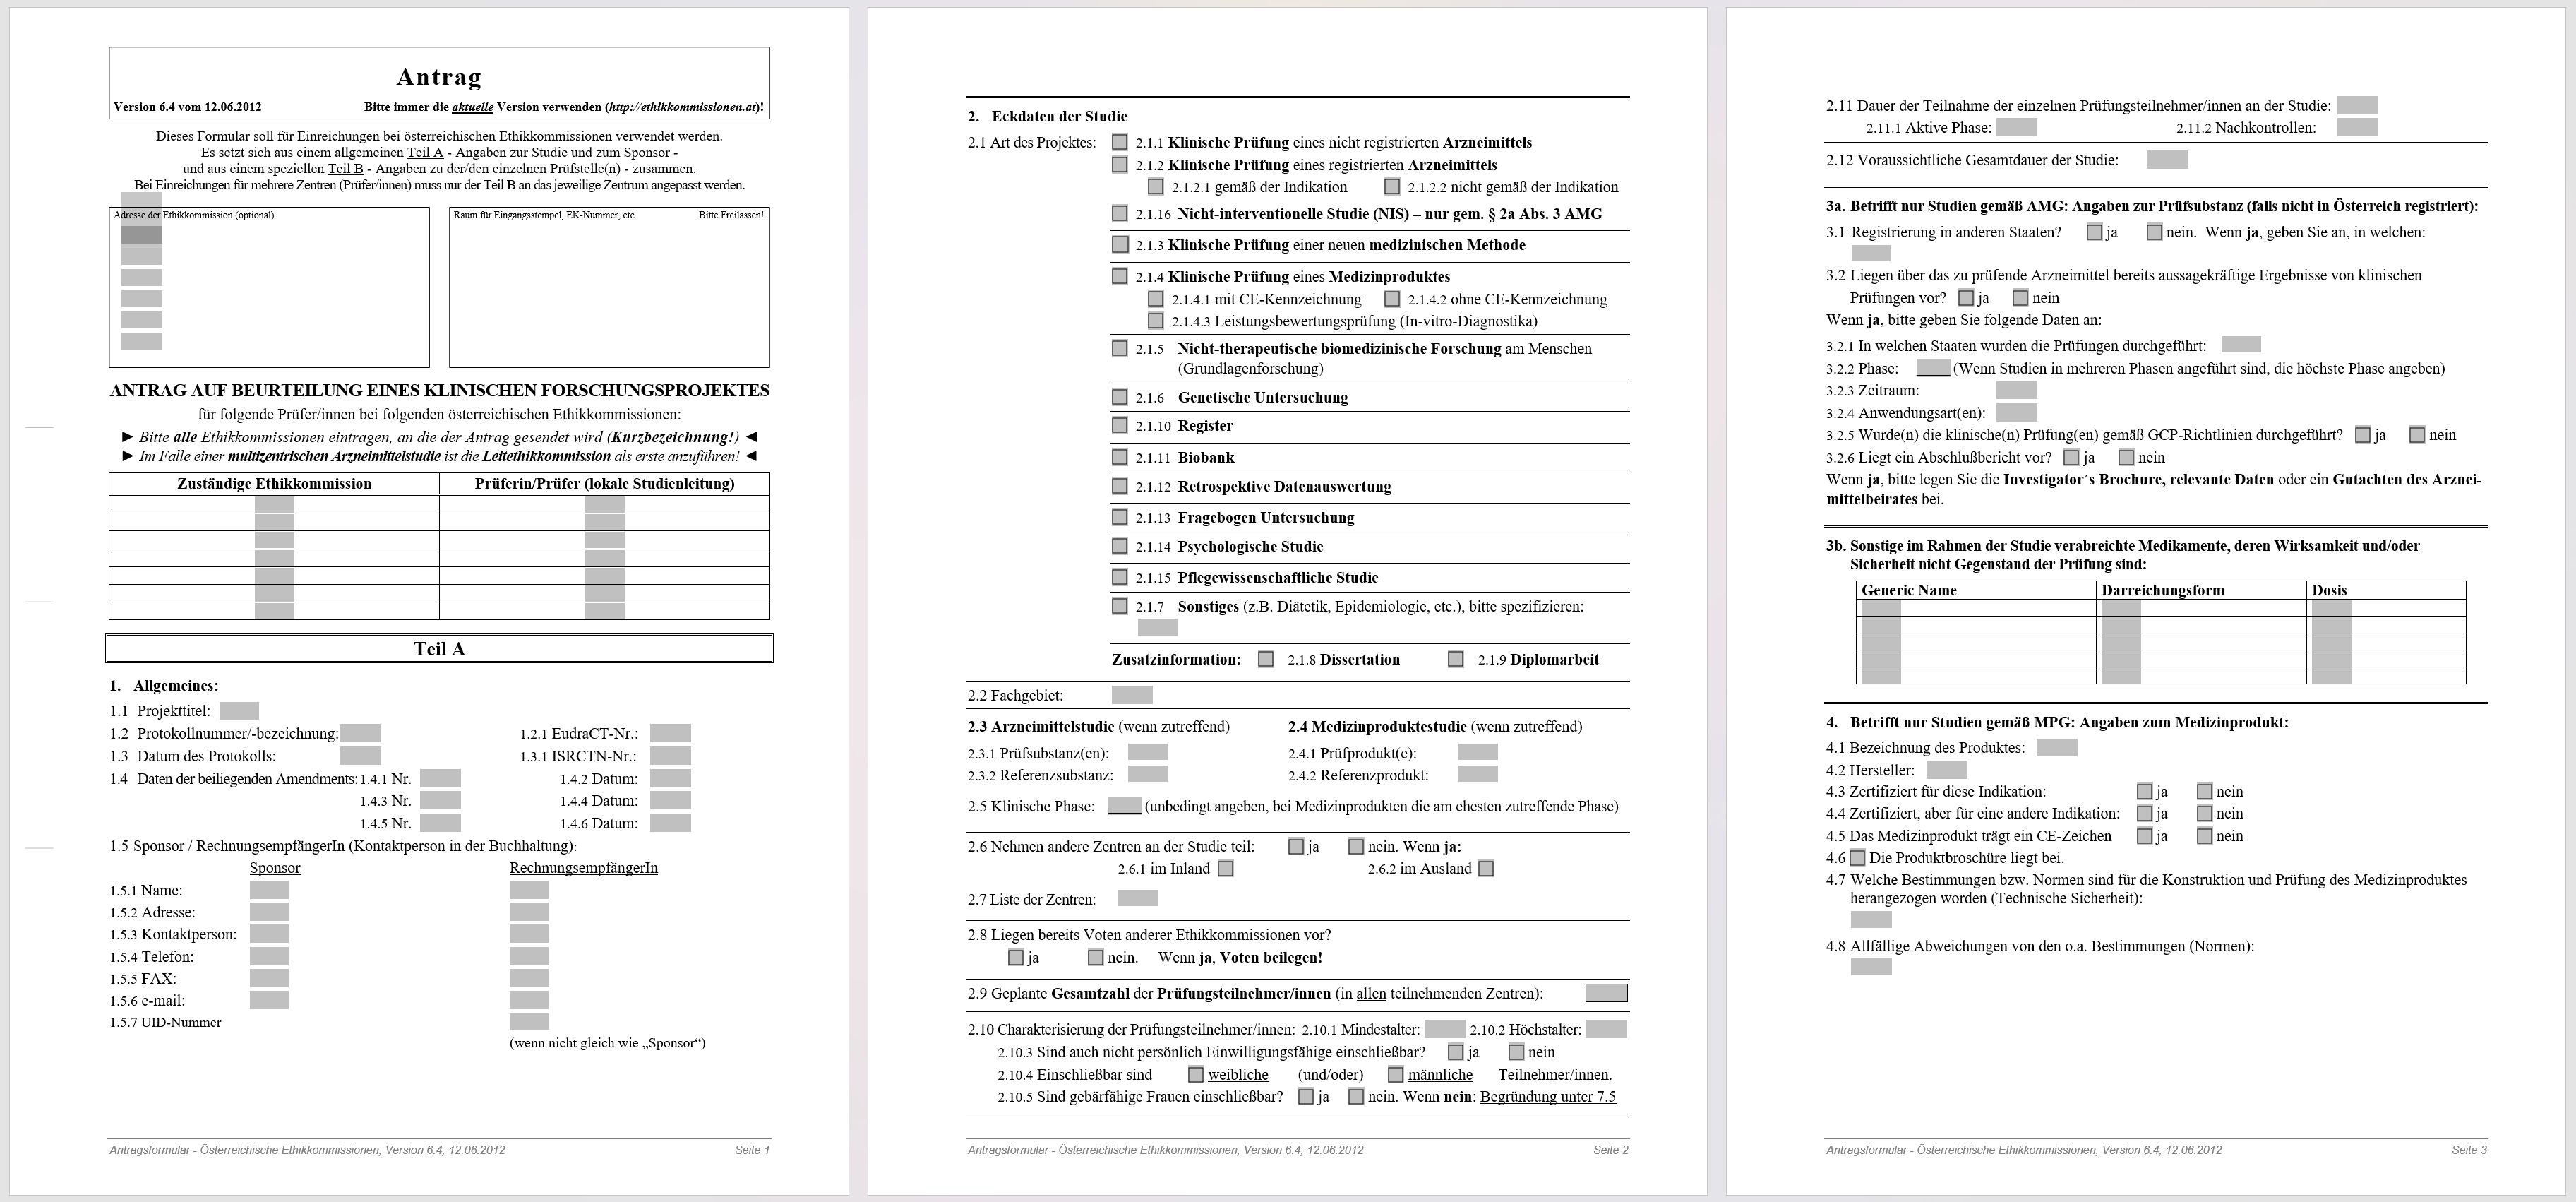
\includegraphics[scale=0.21]{thesis/images/Luidold_Word-Vorlage-Forum-Oesterreichischer-Ethikkommissionen.png}
    \caption[Screenshot der Word-Dokumentenvorlage des Forums Österreichischer Ethikkommissionen]{Screenshot des Antragsformulares auf Basis einer Word-Dokumentenvorlage des \ac{föe} (Quelle: eigene Abbildung)}
    \label{fig:dokumentenvorlage-föe}
\end{figure}

Bei der Durchsicht des Antrages fallen dabei folgende Punkte auf:
\begin{itemize}
    \item Die Vorlage enthält sowohl für die finale Beurteilung benötigte Informationen (die durch die Antragssteller:innen bereitgestellt werden) als auch Ausfüllhilfen und Hilfestellungen, die zwischen den einzelnen Punkten und Fragen eingebettet sind.
    \item Gewisse Tabellen (wie beispielsweise die Tabellen bei Punkt \enquote{6. Angaben zur durchzuführenden Therapie und Diagnostik} auf Seite 5 des Antrages) lassen nur eine gewisse Anzahl an Einträgen zu, ohne den Antragsstellenden die Möglichkeit zu geben, weitere Punkte hinzufügen zu können.
    \item Es stehen keinerlei Formatierungsmöglichkeiten zur Verfügung, um ausgefüllte Informationen beispielsweise mit kursiver oder farbig hinterlegter Schrift zu strukturieren. Alle getätigten Informationen sind automatisch in fetter Schrift angegeben, um sie von der Vorlage unterscheiden zu können.
\end{itemize}

Da das \ac{föe} keine eigene Ethikkommission darstellt, hängt der Prozess des Einreichens des erstellten und ausgefüllten Ethikantrages von der jeweiligen Ethikkommmission ab. Das Forum weißt jedoch darauf hin, dass es trotz der einheitlichen Formulare zusätzliche Anforderungen der Kommissionen geben kann oder das Formular gar nicht mehr in Form der zum Download angebotenen Dokumentenvorlage angenommen wird (für weitere Informationen siehe dazu Kapitel \ref{sub-sec:ecs} ab Seite \pageref{sub-sec:ecs}). \cite{ethikkommission_der_medizinischen_universitat_graz_download_2012}

Aufgrund des inhaltlichen Fokus des \acl{föe} auf medizinische Ethikkommissionen lassen sich aus dem Antrag nur bedingt Anforderungen für den in dieser Masterarbeit auszuarbeitenden Lösungsansatz ableiten. Vor allem aber auch deswegen nicht, da es sich ebenfalls um eine Dokumentenvorlage mit ähnlichen Problemen zur Vorlage der Forschungsethik-Kommission der Fachhochschule Vorarlberg handelt.

\subsection{Vorlage der FH Gesundheitsberufe OÖ}
\label{sub-cec:vorlage-fh-oö}

Das \ac{ieb}\footnote{\href{https://www.fh-gesundheitsberufe.at/f-e/institutionelles-ethikboard/}{Institutionelles Ethikboard der FH Gesundheitsberufe OÖ (\url{https://www.fh-gesundheitsberufe.at/f-e/institutionelles-ethikboard/})}} fokussiert sich auf die Überprüfung ethischer Aspekte bei eingereichten Forschungsprojekten an oder mit Menschen und darauf, ob eine zusätzliche Einreichung bei einer spezialisierten Ethikkommission notwendig ist. \cite{fh_gesundheitsberufe_oo_gmbh_institutionelles_2023}

Das \ac{ieb} greift dabei -- ebenso wie das \ac{föe} und die \ac{fek} der Fachhochschule Vorarlberg -- auf eine Dokumentenvorlage\footnote{\href{https://www.fh-gesundheitsberufe.at/assets/files/IEB-Antragsformular_V1.00_21.09.2022.docx}{Antragsformular Version1 vom 21.09.2022 (\url{https://www.fh-gesundheitsberufe.at/assets/files/IEB-Antragsformular_V1.00_21.09.2022.docx)}}} im mit Microsoft Word kompatiblen \texttt{.docx} Dateiformat zurück. Diese Vorlage wird Antragssteller:innen zum Download angeboten und kann sowohl digital als auch in einer Printversion beim Ethikboard zur Begutachtung eingereicht werden. \cite{fh_gesundheitsberufe_oo_gmbh_einreichung_2023} Abbildung \ref{fig:dokumentenvorlage-ieb} auf Seite \pageref{fig:dokumentenvorlage-ieb} zeigt einen Ausschnitt des Dokumentes, welches mittels Freitext-Feldern und Kontrollkächsten vom Projekttitel bis hin zu detaillierten Fragen zum Studiendesign und Datenschutz abfragt.

\begin{figure}[ht]
    \centering
    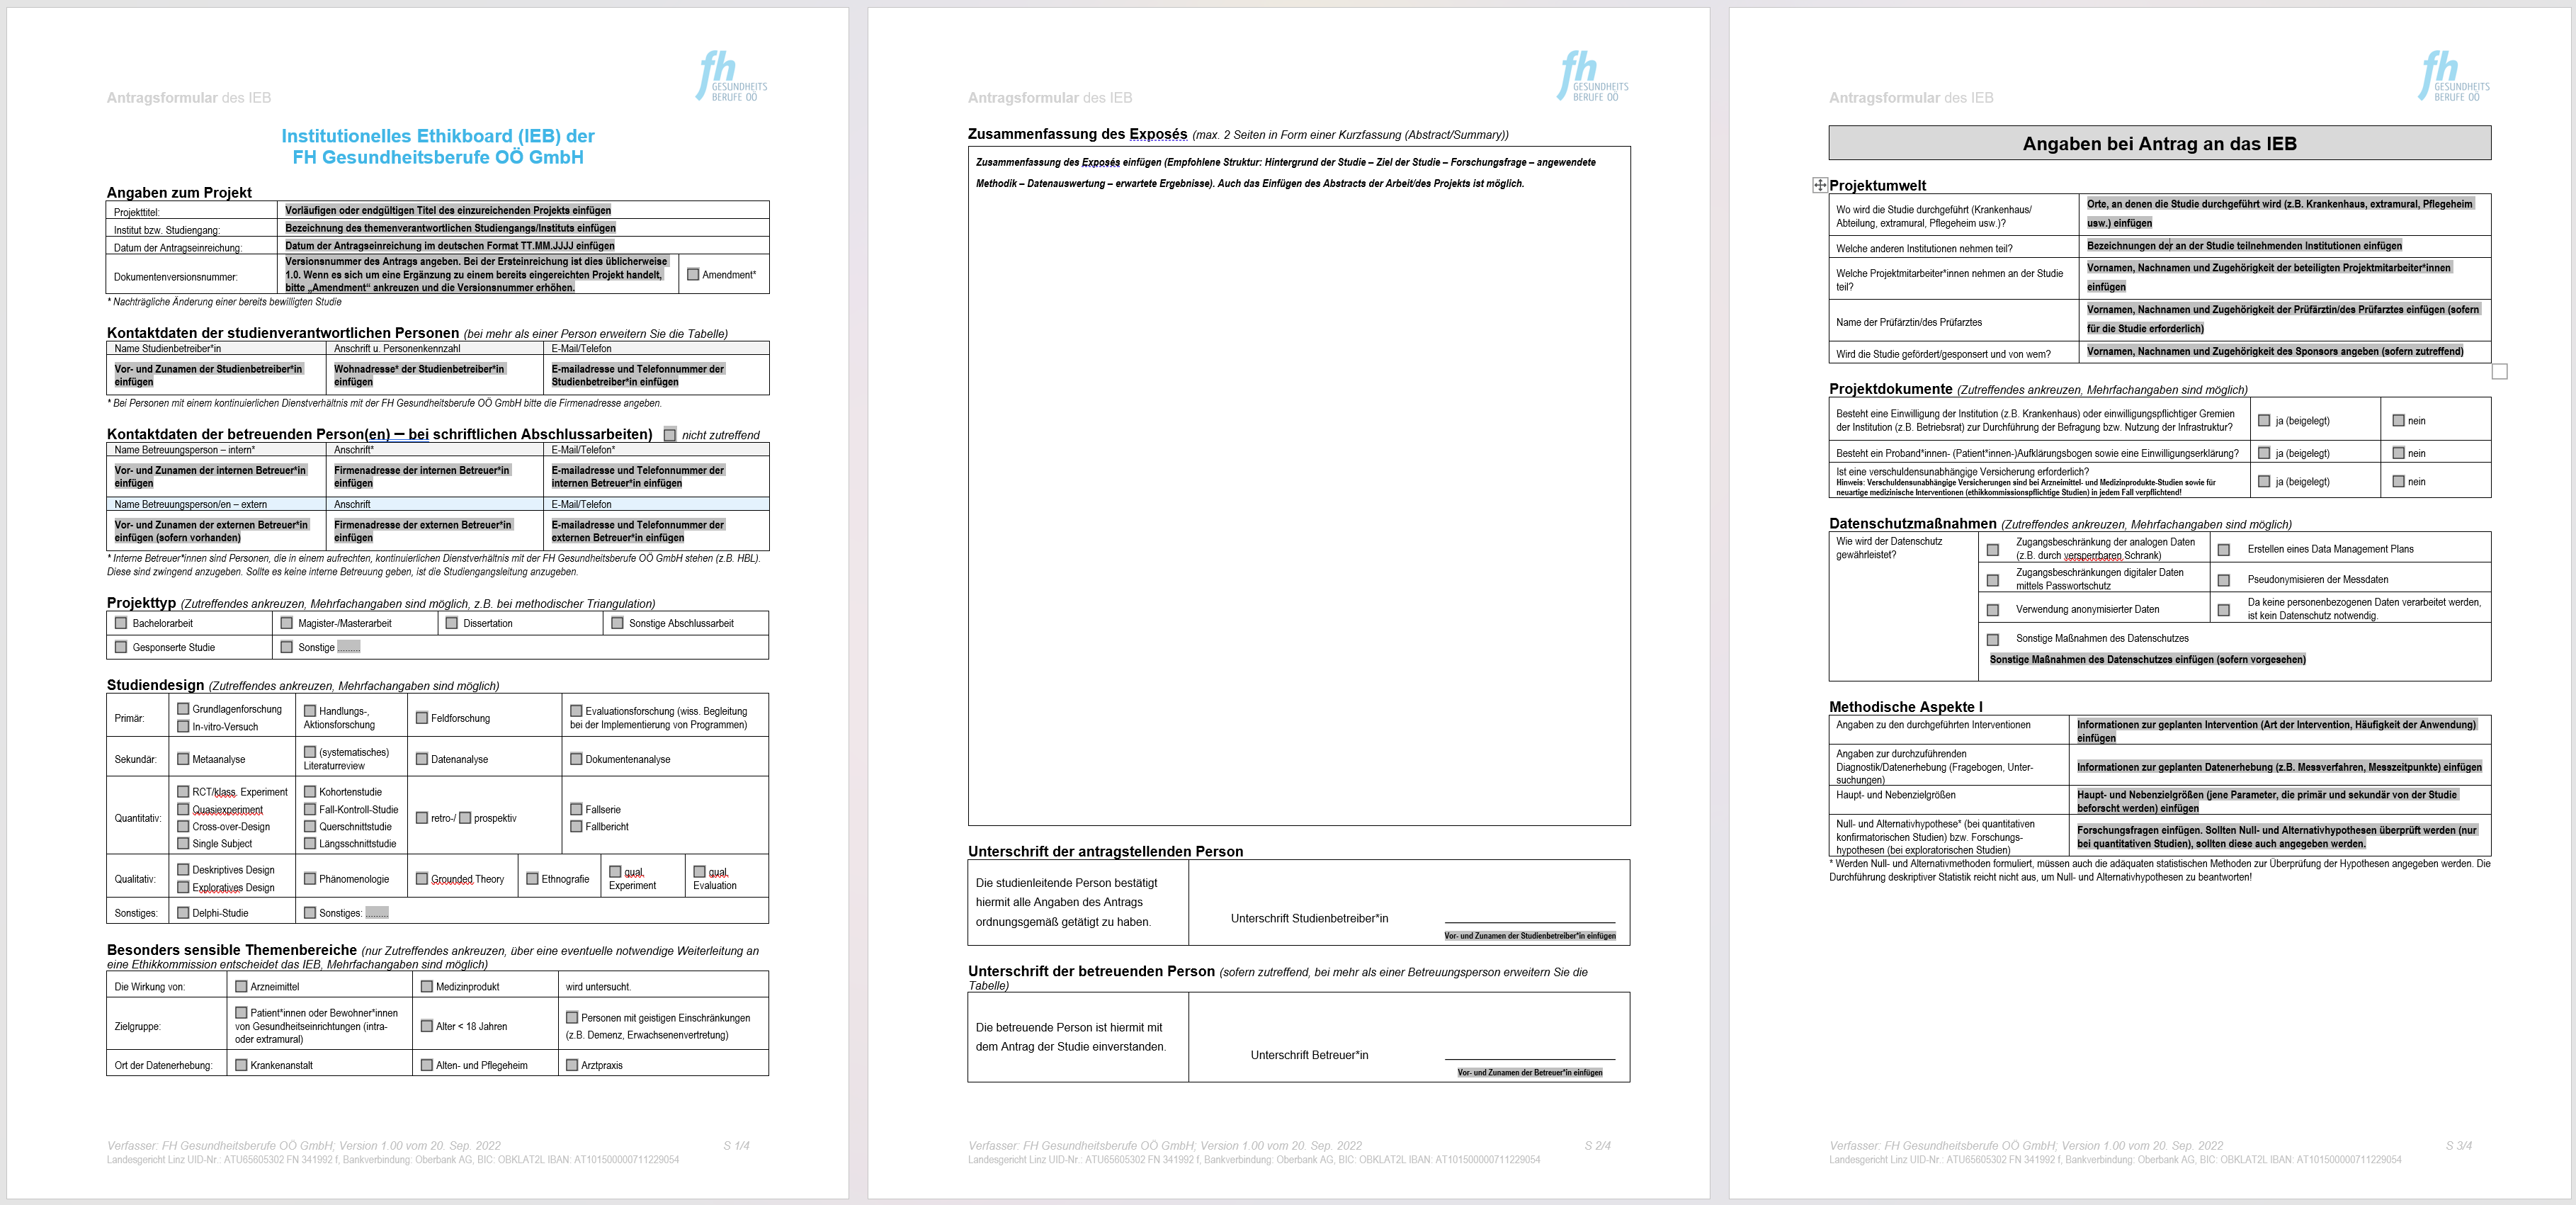
\includegraphics[scale=0.21]{thesis/images/Luidold_Word-Vorlage-IEB-FH-Gesundheitsberufe-OOE.png}
    \caption[Screenshot der Word-Dokumentenvorlage des Institutionellen Ethikboards der FH Gesundheitsberufe OÖ]{Screenshot des Antragsformulares auf Basis einer Word-Dokumentenvorlage des \ac{ieb} (Quelle: eigene Abbildung)}
    \label{fig:dokumentenvorlage-ieb}
\end{figure}

Der Prozess der Einreichung eines Ethikantrages wird vom \ac{ieb} in einen zweistufigen Prozess unterteilt, welcher detailliert in Abbildung \ref{fig:prozess-ethikantrag-ieb} auf Seite \pageref{fig:prozess-ethikantrag-ieb} dargestellt wird. Nach initialer Überprüfung der Vollständigkeit wird der eingereichte Ethikantrag von zwei dem Ethikboard angehörigen Mitgliedern geprüft und entschieden, ob eine direkte Behandlung durch das \ac{ieb} möglich ist oder ob dieser bei einer spezialisierten Kommission eingereicht werden muss. Verläuft die weitere Prüfung positiv, kann dem Antrag entweder eine \enquote{Unbedenklichkeitsbescheinigung} ausgestellt werden oder es findet eine detaillierte Prüfung in einer Vollversammlung des \ac{ieb} statt, die bei Erfülllung etwaiger Auflagen in einem positiven Votum endet. \cite{fh_gesundheitsberufe_oo_gmbh_einreichung_2023}

\medskip

Bei der Durchsicht des Antrages und des Prozesses des \ac{ieb} fallen dabei Punkte auf, die sich stellenweise von den Erkenntnissen zu der in Kapitel \ref{fig:dokumentenvorlage-föe} ab Seite \pageref{sub-sec:vorlage-föe} behandelten Antragsvorlage der \ac{föe} unterscheiden:
\begin{itemize}
    \item Das Antragsformular weicht, trotz des Fokus der Fachhochschule und des \ac{ieb} auf medizinische Studien, sowohl vom Aufbau als auch vom abgefragten Inhalt von der Dokumentenvorlage des \ac{föe} ab.
    \item Die Vorlage enthält zusätzliche Punkte in Form von Ausfüllhilfen und Hilfestellungen, die die Antragsstellenden unterstützen sollen, nicht aber relevant für die finale Beurteilung sind.
    \item Konträr zur Dokumentenvorlage des \ac{föe} ist der Antrag keine strikte Umsetzung eines Formulars, sondern Antragsstellende können das Dokument und alle seine Elemente frei bearbeiten. Dadurch sind Anpassungen sowie auch das Hervorheben von Text mit beispielsweise unterstrichener, kursiver oder farbig hinterlegter Schrift möglich.
\end{itemize}

Das \ac{ieb} erläutert, dass die eigens umgesetzte Dokumentenvorlage gezielt nicht an jene des \ac{föe} angelehnt ist, da sich das Formular des \ac{föe} als zu detailliert und zeitaufwendig in der Bearbeitung herausstellt, sowohl für Antragssteller:innen als auch für die Prüfung selbst. Als zweiter Grund wird auch beziehungsweise vor allem der Umstand genannt, dass vom \ac{ieb} alle Arbeiten geprüft und behandelt werden müssen, die nicht ausschließlich eine Literaturarbeit darstellen. \cite{rosendahl-huber_extern-erfahrungen_2023}

Unabhängig davon sind laut dem \ac{ieb} derzeit zwei digitale Lösungen in Entwicklung, die die aktuelle Word-Dokumentenvorlage längerfristig ablösen sollen, um den Prozess zu vereinfachen und den Arbeitsaufwand sowie auftretende Übertragungsfehler zu minimieren. Eines der aktuell in Ausarbeitung befindlichen Systeme greift dabei auf ein Webformular zurück, das die eingegebenen Daten via E-Mail an das \ac{ieb} übermitteln soll. \cite{rosendahl-huber_extern-erfahrungen_2023}

\begin{figure}[ht]
    \centering
    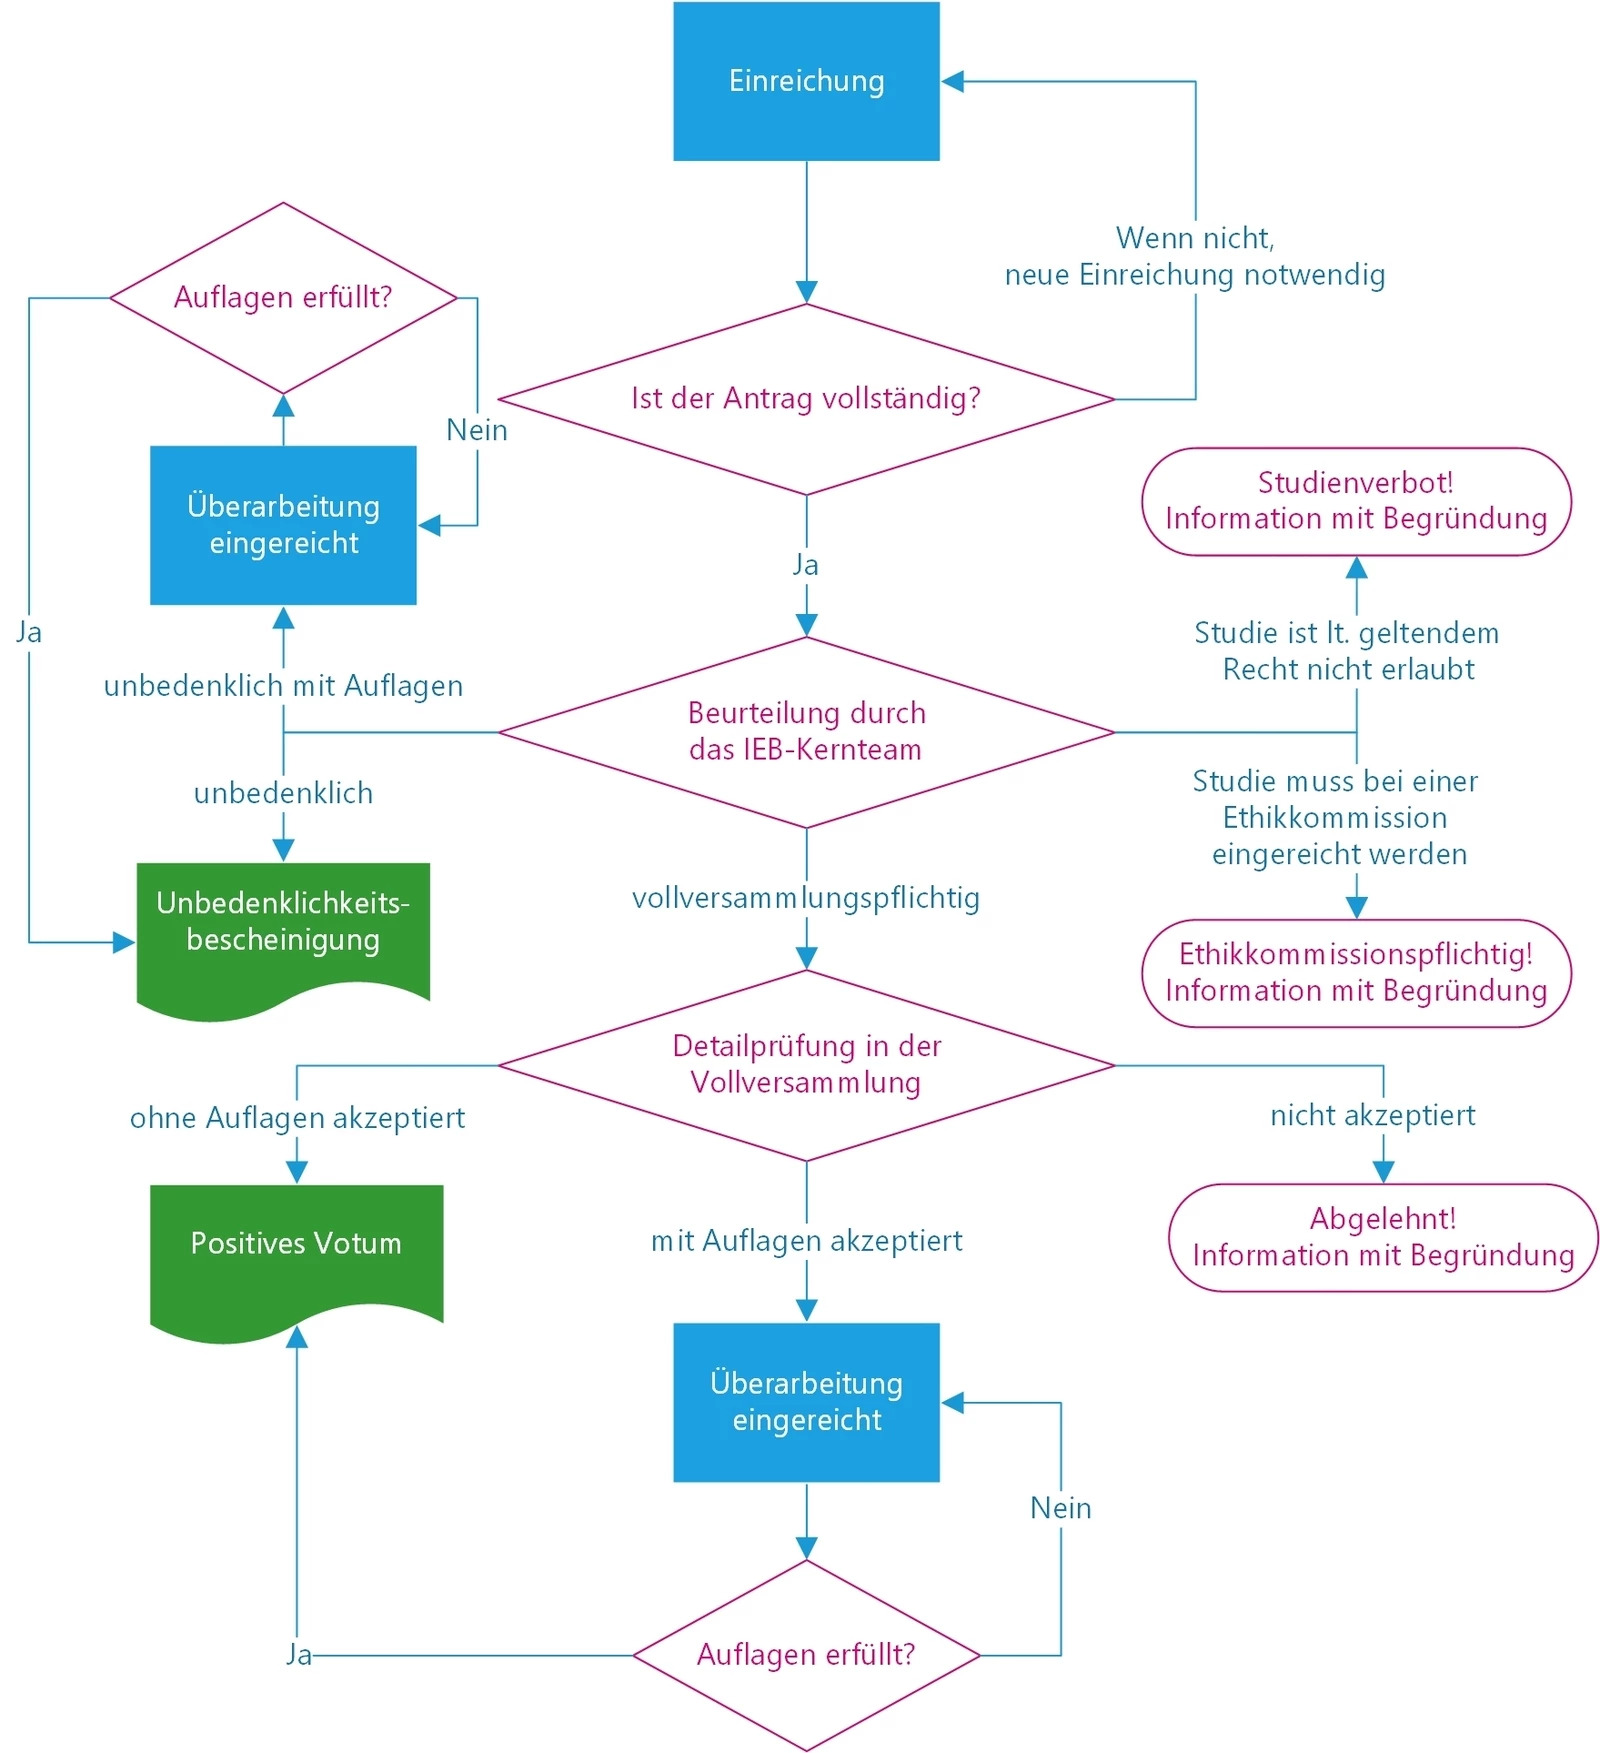
\includegraphics[scale=0.15]{thesis/images/FHGOOE_Prozess-Ethikantrag.jpg}
    \caption[Prozessdiagramm zur Einreichung eines Ethikantrages beim Institutionellen Ethikboard der FH Gesundheitsberufe OÖ]{Prozessdiagramm zur Einreichung eines Ethikantrages beim Institutionellen Ethikboard der FH Gesundheitsberufe OÖ \cite{fh_gesundheitsberufe_oo_gmbh_einreichung_2023}}
    \label{fig:prozess-ethikantrag-ieb}
\end{figure}

Vergleichbar zu der in Kapitel \ref{sub-sec:vorlage-föe} ab Seite \pageref{sub-sec:vorlage-föe} durchgeführten Analyse des \ac{föe} lassen sich auf Basis des Systems des \ac{ieb} keine konkreten Schlüsse für die praktische Ausarbeitung eines neuen Systems ziehen, da ebenfalls eine Dokumentenvorlage zum Einsatz kommt. Als möglicher Anhaltspunkt dient jedoch das in Abbildung \ref{fig:prozess-ethikantrag-ieb} auf Seite \pageref{fig:prozess-ethikantrag-ieb} dargestellte Prozessdiagramm, welches in adaptierter Form in die Neuentwicklung des Systems als Hilfestellung einfließen könnte, um Antragssteller:innen den gesamten Prozess der \ac{fek} der \ac{fhv} übersichtlich darstellen zu können.

\subsection{Einreichplattform der FH Campus Wien}
\label{sub-sec:einreichplattform-fh-campus-wien}

Die FH Campus Wien verfügt seit 2021 über eine eigene Ethikkommission\footnote{\href{https://www.fh-campuswien.ac.at/forschung/ethikkommission-fuer-forschungsaktivitaeten.html}{Ethikkommission für Forschungsaktivitäten \url{https://www.fh-campuswien.ac.at/forschung/ethikkommission-fuer-forschungsaktivitaeten.html}}}, die ihren Ursprung im 2014 an der FH Campus Wien gegründeten Ethik-Komitee hat. Die Ethikkommission unterstützt dabei Forschende bei Anliegen und Fragen im Bereich von ethischen Fragestellungen sowie zu Rechtsvorschriften und Themen, die den Datenschutz betreffen und prüft Forschungsprojekte sowie Forschungsarbeiten auf ethische Aspekte. \cite{fh_campus_wien_ethikkommission_2023}



\subsection{Ethic Commission System (ECS)}
\label{sub-sec:ecs}

todo

\section{Systeme ohne konkreten Bezug}
\label{sec:systeme-ohne-bezug}

todo

% Literaturverzeichnis
\clearpage
\phantomsection
\addcontentsline{toc}{chapter}{Literaturverzeichnis}
\printbibliography

% Anhang
\appendix

\chapter{Eingereichter Ethikantrag}
\label{appendix:eingereichter-ethikantrag}

todo

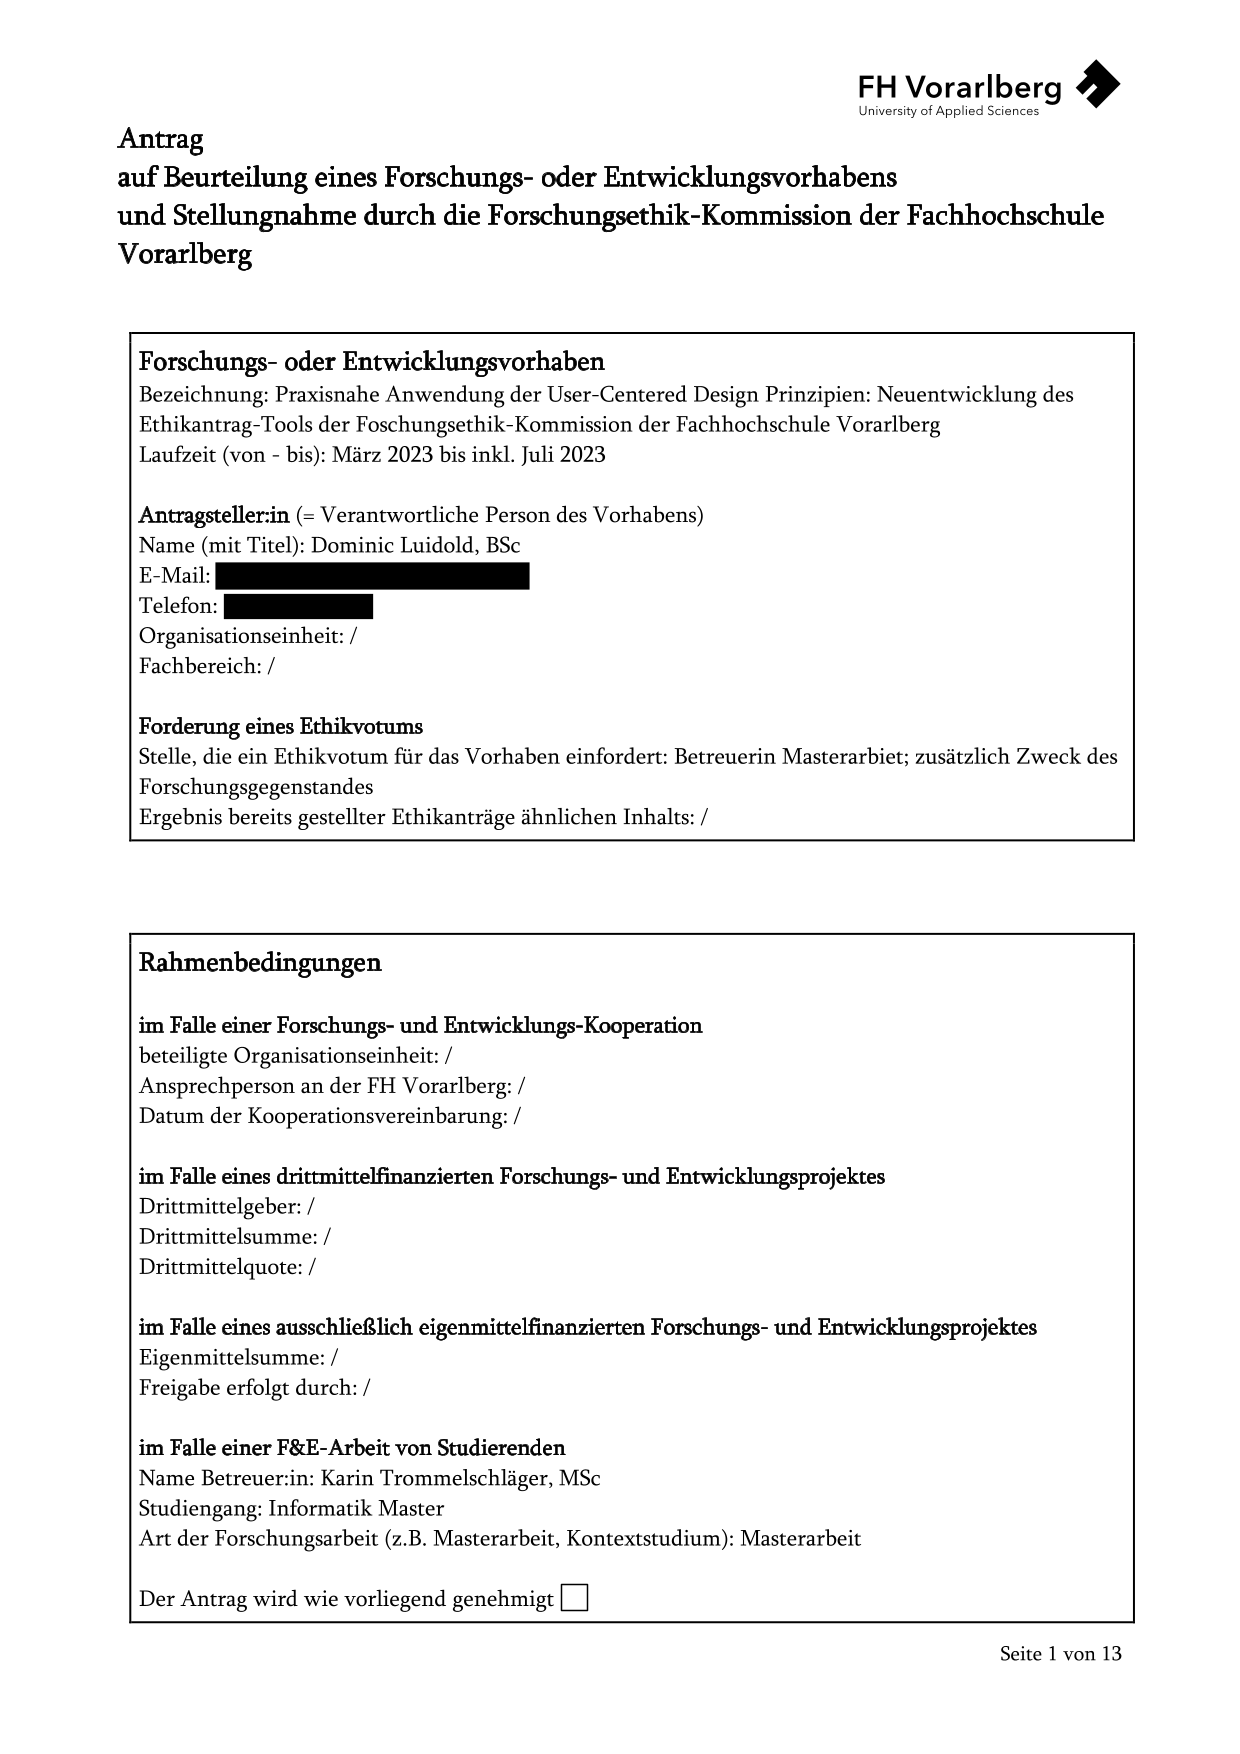
\includepdf[pages=-]{documents/Luidold_Ethikantrag.pdf}

\chapter{Rückmeldung der \acs{fek} zu eingereichtem Ethikantrag}
\label{appendix:rückmeldung-fek}

todo

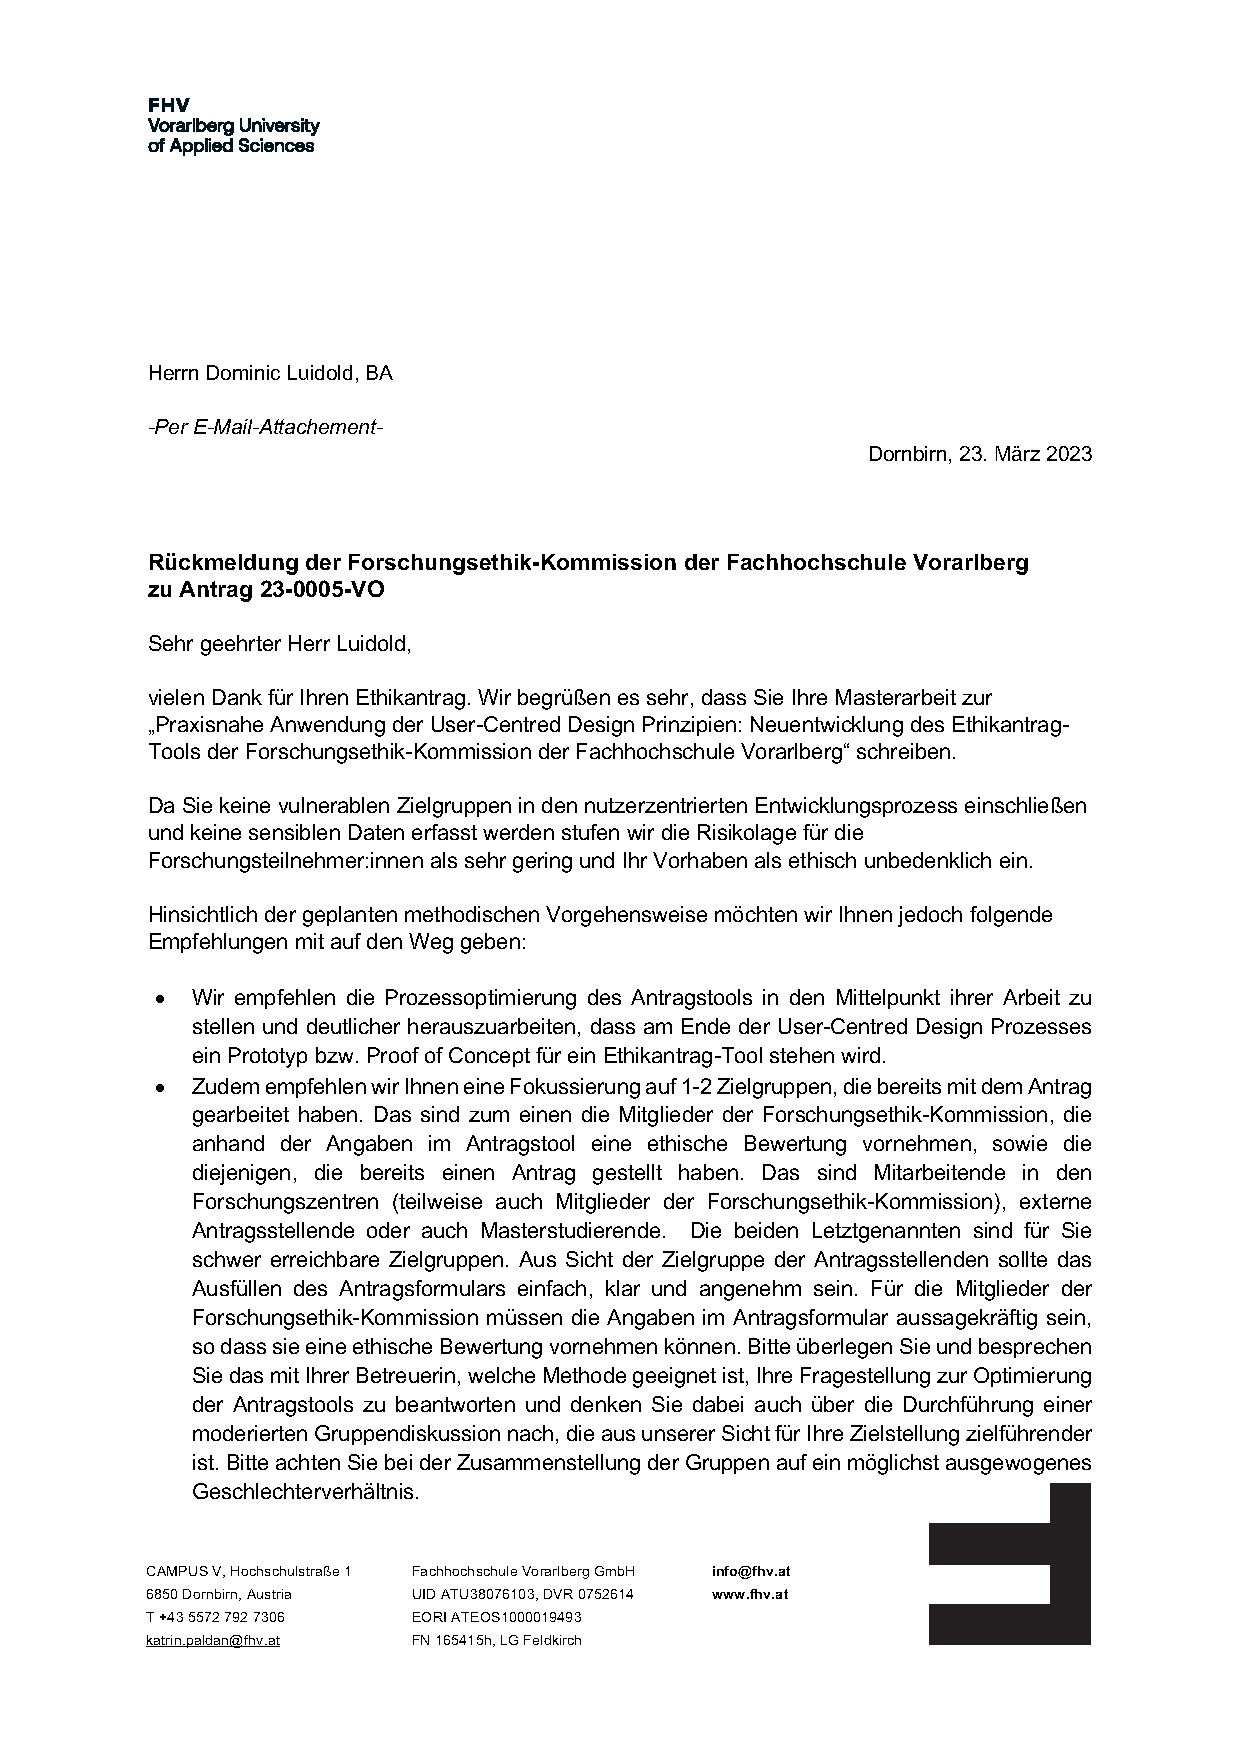
\includepdf[pages=-]{documents/Forschungsethik-Kommission-FHV_Votum-Ethikantrag.pdf}

\chapter{Einwilligungserklärung zur Teilnahme an einem Einzelinterview}
\label{appendix:informed-consent-einzelinterview}

todo

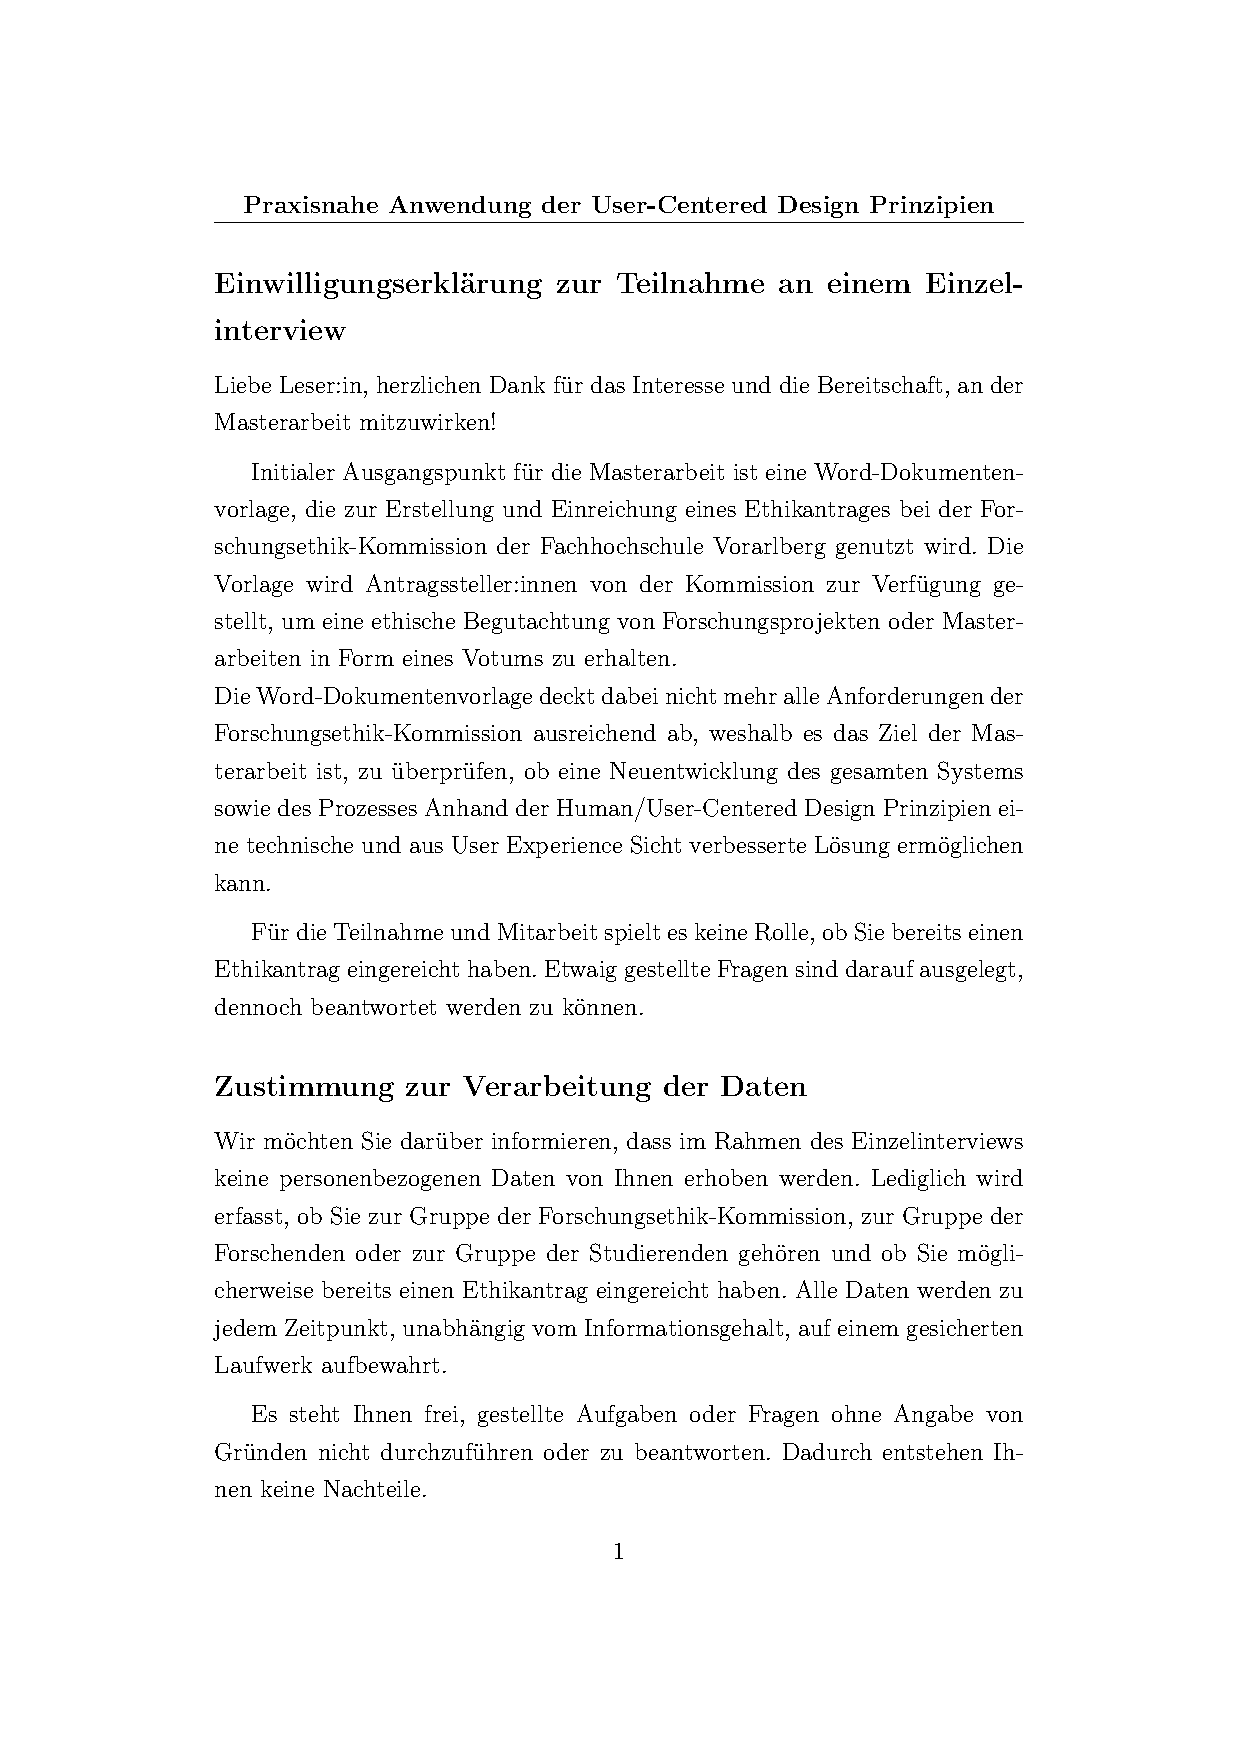
\includepdf[pages=-]{documents/Luidold_Informed_Consent-Einzelinterview.pdf}

\chapter{Einwilligungserklärung zur Teilnahme an einer Gruppendiskussion}
\label{appendix:informed-consent-gruppendiskussion}

todo

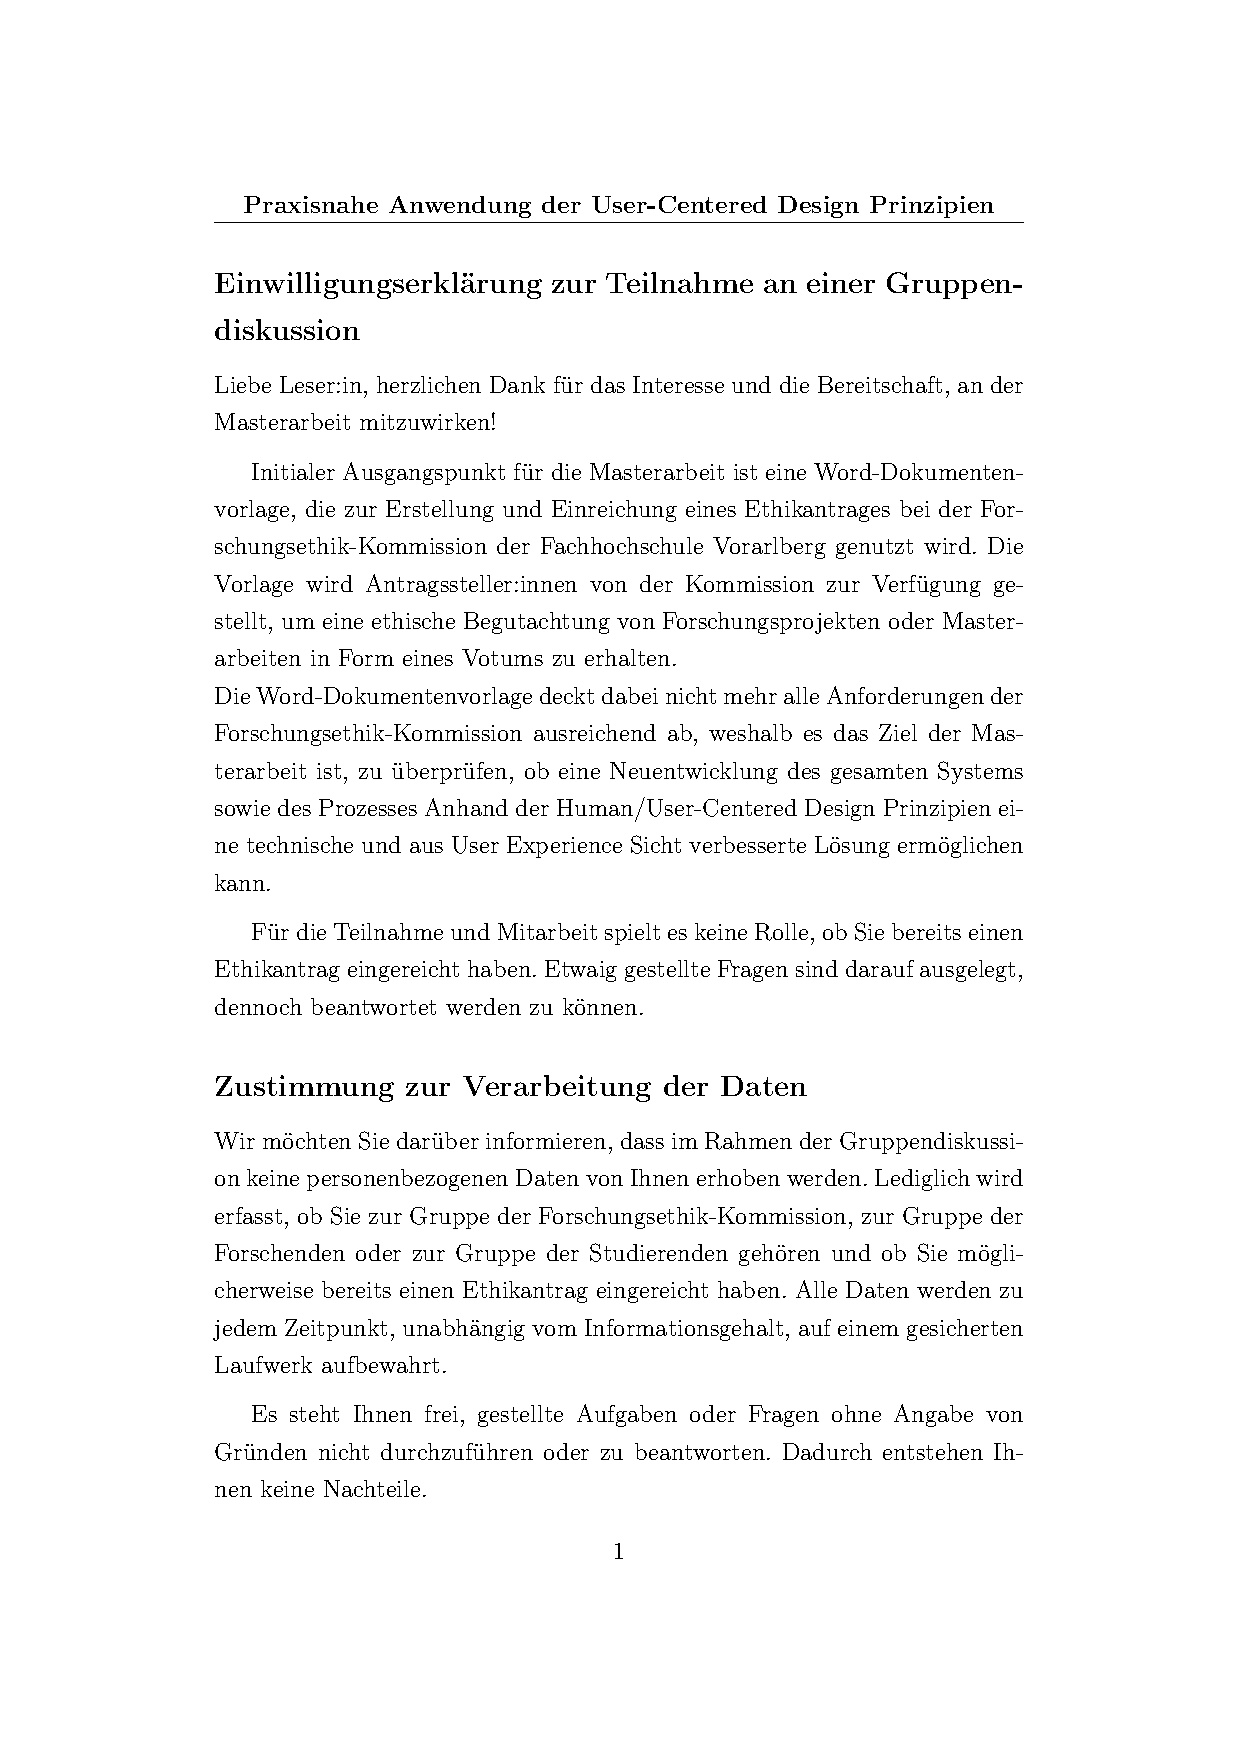
\includepdf[pages=-]{documents/Luidold_Informed_Consent-Gruppendiskussion.pdf}

\chapter{Einzelinterview \#1}
\label{appendix:interview-1}

\section{Informationen zum Interview}
\label{appendix:interview-1-infos}

Das Einzelinterview mit Interviewpartner:in A wurde am Dienstag, den 18.04.23, in den Räumlichkeiten der \ac{fhv} geführt und mittels Tonbandaufnahme aufgezeichnet. Interviewpartner:in A gehört zur Gruppe der Forschenden, die bereits einen Ethikantrag eingereicht haben.

Das Transkript des Interviews enthält beinahe 1:1 das gesprochene Wort, wobei Füllwörter wie beispielsweise \enquote{ähm} etc. der Lesbarkeit halber entfernt wurden. Zusätzlich wurden an zwei Stellen im Transkript Antworten angepasst, um den Datenschutz zu wahren -- diese sind entsprechend gekennzeichnet.

\section{Transkript}
\label{appendix:interview-1-transkript}

\textbf{Dominic:} Gut, also noch einmal auch für die Aufnahme herzlichen Dank, dass Sie sich Zeit nehmen für meine Masterarbeit und mein Interview zum Thema Praxisnahe Anwendung der User-Centered Design Prinzipien im Rahmen der Neuentwicklung des Ethikantrag-Tools für die Ethikkommission der FH Vorarlberg.

Jetzt würde ich direkt schon einmal ganz frech mit der ersten Frage starten die direkt ins Thema hineingeht, und zwar: Warum haben Sie im Rahmen Ihrer Forschungsarbeit überhaupt einen Ethikantrag gestellt?

\textbf{Interviewpartner:in A:} Ja, ich denke wir hätten es eventuell nicht unbedingt machen müssen, aber es waren doch Studierende mit einbezogen, wo eventuell, ja sagen wir, Schaden entstehen hätte können, wenn jemandem schwindelig wird. Wir haben ja Augmented Reality Brillen im Unterricht eingesetzt und weil wir mit Gruppen aus der Schweiz zusammengearbeitet haben, und die Schweizer hätten auf jeden Fall einen Ethikantrag stellen müssen, haben wir als Lead gesagt, wir übernehmen das, da wir selber die Ethikkommission bei uns an der Fachhochschule haben.

\textbf{Dominic:} Okay. Und nachdem Sie den Ethikantrag jetzt gestellt haben und in dem Fall auch den Lead übernommen haben, weil es die Schweizer Kolleg:innen eh gebraucht hätten, können Sie mir einmal den grundlegenden Prozess aus Ihrer Sicht als Antragssteller:in beschreiben, wie denn so ein Ethikantrag abläuft? Von der Erstellung hin bis zur Einreichung einfach die ganzen Schritte, die Sie da vielleicht noch im Kopf haben.

\textbf{Interviewpartner:in A:} Ja, das war jetzt schon wieder relativ lange her. Also ich denke, dass ich Kontakt aufgenommen habe mit \textit{der Ethikkommission}\footnote{Im Interview wurde an dieser Stelle ein konkreter Name genannt. Im Sinne des Datenschutzes findet sich hier eine sinngemäße Verallgemeinerung wieder.} und das ist ja dann das Prozedere, das beschrieben ist, dass es klare Vorgaben gibt. Die habe ich dann alle eingereicht, was notwendig war, und das, was noch gefehlt hat, habe ich in diesem Zeitraum noch nachgereicht und dann gab es ein Feedback, ein Votum von der Ethikkommission und das habe ich beziehungsweise haben wir dann als Gruppe, ich habe das ja nicht alleine gemacht, mit eingearbeitet und die Studierenden informiert und das alles aufeinander abgestimmt. Das, was wir überarbeitet haben, die Änderungen haben wir dann tatsächlich der Ethikkommission noch einmal vorgelegt, sodass sie sehen, dass das, was sie verlangt haben, wir dann auch wirklich geändert haben.

\textbf{Dominic:} Wenn ich das so richtig mitbekommen habe, dann würden Sie sagen, dass der Prozess grundlegend eigentlich schon relativ verständlich ist, wie er momentan abläuft?

\textbf{Interviewpartner:in A:} Grundlegend ist es für mich verständlich gewesen. Es ist natürlich ein Aufwand, aber ich fand es für mich schon klar strukturiert. Ich wusste schon, was ich zu machen hatte und ich denke, dass es schon auch gerechtfertigt ist von der Ethikkommission einen gewissen Level oder Standard einzuhalten, den man auch erbringen muss, denn es ist ja auch ein Gütesiegel, das sie vergeben. Ich weiß nicht mehr, ob mir im Einzelnen etwas unklar war, aber wenn habe ich mich an \textit{die Ethikkommission}\footnote{Im Interview wurde an dieser Stelle ein konkreter Name genannt. Im Sinne des Datenschutzes findet sich hier eine sinngemäße Verallgemeinerung wieder.} gewandt und nachgefragt. Aber es ist schon klar beschrieben.

\textbf{Dominic:} Und gerade eine Frage dazu: In dem Fall, nachdem der Prozess für Sie nicht unbedingt unverständlich war, würden Sie trotzdem vielleicht Punkte daran ändern oder sagen Sie der Prozess an sich ist soweit eigentlich klar oder in sich schlüssig oder sehen Sie da, als jemand der wirklich einen Antrag gestellt hat, aus der Perspektive als Antragssteller:in Punkte die Sie einfach noch einmal anders handhaben würden, wenn Sie persönlich in der Forschungsethik-Kommission wären?

\textbf{Interviewpartner:in A:} Puh. Das weiß ich jetzt eigentlich auch nicht mehr. Ich denke, ich glaube es ist alles in Papierform gelaufen beziehungsweise Dateien hin und her geschickt. Vielleicht wäre das eine Vereinfachung, wenn man das alles in digitaler Form einreichen kann, dass das nicht per E-Mail hin und her geschickt werden muss. Das wäre vielleicht eine Möglichkeit, wie man den Prozess vereinfach könnte.

\textbf{Dominic:} Dann würden Sie einfach klar sagen, das Hin- und Herschicken der Word-Dokumentenvorlage die es gibt, dass das in einer digitaleren Form, wenn das vorhanden wäre, das würde helfen.

\textbf{Interviewpartner:in A:} Ja, genau.

\textbf{Dominic:} Nachdem Sie jetzt gerade den Prozess beschrieben haben, würden Sie wieder einen Ethikantrag stellen, wenn es Projekte gibt, bei denen es die Umstände zulassen?

\textbf{Interviewpartner:in A:} Ja, klar. Ich denke, dass das eine feste Institution oder feste Größe ist und Gott sei Dank haben wir das in der Zwischenzeit. Und da wir jetzt im Studiengang und im Forschungszentrum immer entweder mit Studierenden oder Patient:innen, Bewohner:innen, Menschen und Angehörigen zu tun haben, denke ich, wird das auch in der Zukunft vermutlich noch mehr gefragt und dass das einfach auch Zeit, Stunden und Geld ist, das man mit einkalkulieren muss und das schon machen wird. Also ich möchte nicht per se sagen, wir lassen das. Ich frage das ja auch bei Studierenden, die dementsprechende Bachelor- oder Masterarbeiten machen, an, ob sie da ein Votum von der Ethikkommission brauchen, wenn dementsprechend Gruppen mit involviert sind.

\textbf{Dominic:} Gibt es vielleicht dennoch Gründe, warum Forschende sich hier an der FH nicht dazu entscheiden einen Ethikantrag zu stellen? Oder vielleicht gerade auch weil Sie die Studierenden erwähnt haben, gibt es dort vielleicht irgendwelche Gründe, abgesehen vom vielleicht Zeitaufwand oder ist es vielleicht sogar der Zeitaufwand?

\textbf{Interviewpartner:in A:} Ja, also Gründe vielleicht dass es im Forschungsdesign nicht zwingend verlangt wird, und wenn es nicht zwingend verlangt wird, dann machts niemand und wenn es nicht verlangt ist, dass viele vielleicht denken: \enquote{Ja, das ist überhaupt nicht notwendig. Ich mache nichts, was ethisch kritisch sein könnte. Ich werde niemandem Schaden zufügen, es hat jeder die Möglichkeit entweder in die Gruppe oder die Gruppe zu kommen oder davon zu profitieren.} Im Endeffekt dass dieses Verständnis, das könnte ich mir vostellen, nicht in allen Fachbereichen, in allen Disziplinen ausreichend vorhanden ist und dass das mehr und mehr auch in der Lehre thematisiert und sensibilisiert werden sollte. Oder wie kürzlich die \textit{forward}\footnote{Anmerkung: \href{https://www.fhv.at/forward-event/}{Event-Format der Fachhochschule Vorarlberg (\url{https://www.fhv.at/forward-event/})}} stattgefunden hat, dass das einfach schon ein Thema ist und auch sensibilisiert wird dafür.

\textbf{Dominic:} Also würden Sie konkret zusammenfassen, dass es mehr externe Faktoren sind als die Arbeit oder der Prozess der Ethikkommission selbst?

\textbf{Interviewpartner:in A:} Würde ich schon sagen. Es hat auch etwas mit der Haltung des Einzelnen zu tun. Und wenn es den Prozess selber erleichtern würde, oder wie der Prozess ist, ob der aufwendig ist, schwierig, das merkt jemand, ein Antragssteller, erst dann, wenn er es tatsächlich macht und er hat dann ja nicht unbedingt einen Vergleich damit oder tatsächlich mit den Auflagen oder dem Votum, das dann die Ethikkommission abgibt. Ich würde so spontan sagen, dass wenn jemand einen Antrag stellt, dass es dann gut ist, dass das Prozedere, der Ablauf und alles, was es zu machen gibt, so einfach wie möglich ist und dass man das mit allen möglichen Designs und Technologien, und auch mit dem, was Sie vielleicht beabsichtigen, verbessern könnte, ja? Aber dass das letztendlich, diese Perfektion und von dem, was man verändert, glaube ich nicht unbedingt etwas daran ändert, ob mehr oder weniger Anträge gestellt werden. Ich glaube jetzt auch nicht, dass das der Eine oder der Andere Ethikkommission A und B, die an anderen Hochschulen oder Universitäten oder irgendwo anders sind, dass man die vergleicht. Ich kenne es von Deutschland her, dass man vielleicht schaut: wo ist es am einfachsten, wo ist der Aufwand gering oder wie viel kostet es, wie schnell geht es, dass ich irgendwo meinen Antrag durchbekomme. Teilweise kostet es ja auch wirklich Geld, das wissen wir vielleicht, oder viele, gar nicht zu schätzen, dass das aktuell oder gar nie irgendetwas kostet hier an der Fachhochschule. Aber es gibt schon auch Ethikkommissionen, wo man wirklich auch Geld zahlen muss, das dann auch im Budget vom Forschungsprojekt mit vorgesehen ist.

\textbf{Dominic:} Sie haben ganz zu Beginn des Interviews schon die Dokumente, die per E-Mail hin und her geschickt werden, angesprochen, die nicht unbedingt optimal sind, wenn man das so sagen kann. Es ist eine Dokumentenvorlage, die natürlich mit Microsoft Word kompatibel ist und natürlich auch mit den anderen, größeren freien Texteditoren. Was waren dort vielleicht Ihre konkreten Erfahrungen mit der Dokumentenvorlage? Haben Sie das noch im Kopf?

\textbf{Interviewpartner:in A:} Also, ich muss sagen, nicht wirklich.

\textbf{Dominic:} Gibt’s in dem Fall nichts, das Sie, nachdem der Antrag schon länger her ist..

\textbf{Interviewpartner:in A:} .. wo ich jetzt sagen könnte, das und das.

\textbf{Dominic:} Genau. Ob Ihnen vielleicht noch etwas im Kopf geblieben ist, was ist positiv aufgefallen oder eher negativ.

\textbf{Interviewpartner:in A:} Im Normalfall kann ich mich schon daran erinnern, wenn irgendein Dokument, an dem ich gearbeitet habe, wenn ich das mit dem Mac verwende, irgendwie nicht zu benutzen ist oder nicht funktioniert, wenn es zu bearbeiten ist, wenn wir es innerhalb der Gruppe wieder hin und her schicken. Nein, also mir fällt nichts ein.

\textbf{Dominic:} Das finde ich ganz interessant eigentlich, weil gerade, wenn einem etwas konkret einfällt und so spontan, dann muss es stark aufgefallen sein.

\textbf{Interviewpartner:in A:} Ja, genau, ja.

\textbf{Dominic:} Vielleicht jetzt noch die letzte Frage, das Interview ist tatsächlich gar nicht so lange. Nachdem Sie jetzt wissen, dass ich mich mit meiner Masterarbeit mit dem ganzen Thema beschäftige, was die Anforderungen sind, was die Wünsche sind, sowohl aus Sicht der Kommission als auch aus Sicht der Antragssteller:innen. Sie haben es eh schon erwähnt, die Word-Dokumente, die Sie herunterladen und per E-Mail verschicken sind nicht ganz optimal. Gibt es irgendetwas, dass Sie sich ganz konkret wünschen würden, wo Sie sagen, wenn Sie wieder einen Ethikantrag ausfüllen, dann würde Ihnen das das Ganze noch einmal erleichtern oder vielleicht auch Hilfestellungen, die Sie sich während dem Ausfüllen gewünscht hätten oder Beispiele oder irgendetwas in die Richtung?

\textbf{Interviewpartner:in A:} Ich weiß jetzt nicht, ob das hier passt, aber dass es vielleicht auch Textbausteine gibt. Nein, das wird nicht funktionieren. Meistens wird es ja beantwortet aus meinem Forschungsdesign heraus. Also nicht wirklich etwas. Es ist schon etwas her.

\textbf{Dominic:} Das ist vollkommen in Ordnung. Vielleicht hätten Sie gesagt, es soll ein Online-Formular sein, dass das Ganze ablöst und vereinfacht, oder bei der Dokumentenvorlage bleiben, weil man dort die meisten Freiheiten hat, aber bei einer Dokumentenvorlage die weniger strikt ist wie die aktuelle Word-Dokumentenvorlage. Aber wenn Sie keine konkreten Wünsche haben, dann passt das eh ganz gut. 

Soweit ich das sehen kann, waren das schon meine Fragen, ganz kurz und bündig. Dann möchte ich mich für das Interview bedanken und wünsche Ihnen noch einen schönen Tag und eine schöne Mittagszeit.

\textbf{Interviewpartner:in A:} Danke.

\chapter{Einzelinterview \#2}
\label{appendix:interview-2}

\section{Informationen zum Interview}
\label{appendix:interview-2-infos}

Das Einzelinterview mit Interviewpartner:in B wurde am Mittwoch, den 19.04.23, in den Räumlichkeiten der \ac{fhv} geführt und mittels Tonbandaufnahme aufgezeichnet. Interviewpartner:in B gehört zur Gruppe der Forschenden, die bereits einen Ethikantrag eingereicht haben.

Das Transkript des Interviews enthält beinahe 1:1 das gesprochene Wort, wobei Füllwörter wie beispielsweise \enquote{ähm} etc. der Lesbarkeit halber entfernt wurden. Zusätzlich wurden an zwei Stellen im Transkript Antworten angepasst, um den Datenschutz zu wahren -- diese sind entsprechend gekennzeichnet.

\section{Transkript}
\label{appendix:interview-2-transkript}

\textbf{Dominic:} Okay, die Aufnahme läuft. Vielen Dank für die Bereitschaft beim Interview für meine Masterarbeit mit dem vorläufigen Arbeitstitel Praxisnahe Anwendung der User-Centered Design Prinzipien am Beispiel der Neuentwicklung des Ethikantrag-Tools der Fachhochschule Vorarlberg mitzuwirken.

Ich würde jetzt direkt einfach mit der ersten Frage ganz frech schon starten: Warum hast du denn einen Ethikantrag gestellt?

\textbf{Interviewpartner:in B:} Weil wir Forschung mit Menschen machen und es da eben wichtig ist, zu berücksichtigen, ob da Risiken auftreten und was das eben für Folgen haben könnten.

\textbf{Dominic:} In dem Fall für dich ganz klar gewesen oder für euch im Forschungsprojekt, dass da ein Ethikantrag wirklich notwendig ist.

\textbf{Interviewpartner:in B:} Ja, gerade wenn es um Menschen geht. Es ist natürlich immer etwas schwierig, ab wann braucht man sowas, braucht man für einen normalen Usability-Test einen Ethikantrag? Also da sind die Grenzen schon noch etwas schwammig und da wär eine Unterstützung von einem Tool sicher hilfreich das zu entscheiden, ob es überhaupt einen Ethikantrag braucht.

\textbf{Dominic:} Okay. Dann würde ich direkt mit der nächsten Frage weitermachen, und zwar: Nachdem jetzt eigentlich relativ klar war, dass ein Ethikantrag gestellt werden muss, weil eben Menschen involviert sind, würde mich interessieren, wie denn die Schritte aus Sicht eines:einer Antragssteller:in, also aus deiner Sicht, aussehen, die man durchläuft, wenn man Ethikantrag einreicht? Wie da der Prozess so ist?

\textbf{Interviewpartner:in B:} Also konkret in meinem Fall war es so, man lädt sich den Antrag runter, liest den durch, stellt fest, dass man da allerhand anderer Dinge noch vorbereiten muss damit man den Antrag ausfüllen kann und ja, bearbeitet nach und nach die Punkte, die dafür notwendig sind. Was ganz wichtig ist, ist eben, dass das Forschungsdesign schon vorher ziemlich detailliert ausgearbeitet sein muss, damit man den Antrag überhaupt ausfüllen kann.

\textbf{Dominic:} Der weitere Ablauf, im Sinne was passiert wenn der Ethikantrag bei der Kommission eingereicht wurde und wie dann der Ablauf für dich als Antragssteller:in ist, das ist soweit in dem Fall auch verständlich?

\textbf{Interviewpartner:in B:} Das war relativ klar dass da dann die Ethikkommission zusammentreten muss, also zunächst begutachtet werden muss von den einzelnen Mitgliedern und dann irgendwann einmal das Feedback kommt.

\textbf{Dominic:} Nachdem wir jetzt eben kurz abgeklärt haben, warum man einen Ethikantrag stellen sollte oder warum ihr einen Ethikantrag gestellt habt und wie der Prozess so abläuft, würdest du wieder einen Ethikantrag stellen, eben mit dem Wissen, wie der gesamte Prozess abläuft?

\textbf{Interviewpartner:in B:} Ja, auf jeden Fall. Also wenn es wieder die Voraussetzungen gibt, dass mit Menschen geforscht wird und da eventuell Risiken verknüpft sind, dann ist das auf jeden Fall hilfreich da einen Antrag zu stellen. Es geht auch darum, dass man selber das Feedback bekommt, was man vielleicht verbessern sollte am Forschungsdesign, falls Risiken nicht korrekt berücksichtigt sind.

\textbf{Dominic:} Okay. Nachdem wir jetzt das kurz einmal zusammengefasst haben, gibt es konkrete Punkte, die du jetzt am Prozess vielleicht verändern würdest, einfach weil du weißt, wie der Ethikantrag aussieht, wie er auszufüllen ist, was es da für Anforderungen gibt, wie der weitere Prozess aussieht.

\textbf{Interviewpartner:in B:} Ja, ich würde es begrüßen wenn, man kein Word-Formular mehr ausfüllen muss, sondern dass man da ein bisschen durchgeleitet wird durch den Prozess. Also es sind auch einige Dinge die einem so vorkommen zumindest, dass sie doppelt ausgefüllt werden müssen, je nachdem, ob es ein Produkt wird oder ob es nur eine Forschung ist, dass man da unterschiedliche Blätter ausfüllen muss.

\textbf{Dominic:} Was die Dokumentenvorlage abfragt, wiederholt sich dann in diesem Fall stellenweise aus deiner Sicht?

\textbf{Interviewpartner:in B:} Genau. Also je nachdem, ob es ein Produkt ist oder eine Forschung muss man unterschiedliche Dinge ausfüllen, die aber meistens schon davor einmal erwähnt wurden.

\textbf{Dominic:} Gibt es sonst noch etwas, was dir bei der Dokumentenvorlage oder auch generell im Prozess aufgefallen ist oder an dem wie die Fragen gestellt werden oder was abgefragt wird, wo du etwas abändern würdest?

\textbf{Interviewpartner:in B:} Ja, also eh schon kurz angesprochen. Die erste Entscheidung ist:Muss ich überhaupt einen Ethikantrag stellen? Da wäre es cool, wenn es irgendein Hilfsmittel gibt, das abzuschätzen. Es ist schon klar, dass es im Endeffekt immer von der Kommission vielleicht entschieden werden muss. Je nachdem, in Grenzfällen, aber es gibt vorgelagert sicher Möglichkeiten wo man das abfangen kann, wenn ich technische Messungen irgendwo durchführe wo keine Menschen involviert sind, dann kann es zwar zur Technikfolgeabschätzung vielleicht sinnvoll seinen einen zu stellen, aber jetzt nicht unbedingt unmittelbar weil Menschen gefährdet sind.

\textbf{Dominic:} Da wir eigentlich den ganzen Prozess schon relativ gut angesprochen haben, auch was du konkret jetzt in deinem Fall verbessern würdest was dir aufgefallen ist, gibt es vielleicht Anlässe, die dir aufgefallen sind oder dir einfallen könnten, die Forschende aktiv davon abhalten, einen Ethikantrag zu stellen, obwohl diese vielleicht auch wirklich einen Ethikantrag in Betracht gezogen haben?

\textbf{Interviewpartner:in B:} Das erste ist vielleicht, dass sie nicht wussten, dass es überhaupt eine Ethikkommission gibt an der FH. Das heißt, alleine dafür wäre schon so ein Tool sinnvoll, das man verbreiten kann. Das könnte dann zum Beispiel in den Bachelor- und Masterseminaren angesprochen werden, dass man da draufgeht um einen Check zu machen, brauch ich überhaupt einen Ethikantrag oder nicht, um da eben die Awareness zu schaffen, dass es so etwas überhaupt gibt. Ich weiß nicht, ob das sowieso stattfindet.

\textbf{Dominic:} Das wäre sicherlich sinnvoll, ja.

\textbf{Interviewpartner:in B:} Vom Prozess selber, wenn man entschieden hat, man will einen Ethikantrag stellen, momentan muss man eben das Word-Formular ausfüllen, das es einem teilweise schwer macht. Ich weiß allerdings nicht ob das ein Mac-spezfisiches Problem ist, aber zum Beispiel will ich etwas hineinschreiben und dann springt der Cursor gleich zum nächsten Feld, ich kann da gar nichts hineinschreiben, wenn ich nicht ganz genau an den Start klicke. Solche Sachen.

\textbf{Dominic:} Also wirklich nicht nur von der Fragestellung her sondern rein von der Bedienung schon.

\textbf{Interviewpartner:in B:} Rein von der Bedienung, aber ich denke das ist in der neuesten Version behoben. Aber das ist ja nur ein Teil, das heißt man bekommt ja darauffolgend, also man reicht den ein und wartet bis man Feedback bekommt. Da wäre es interessant, wenn es so eine Prozessansicht geben würde, wo man sieht, wo steckt der Antrag gerade, er ist jetzt in Begutachtung, die Kommission muss zusammentreffen und das nächste Treffen findet dann und dann statt.

\textbf{Dominic:} Also dass man ein bisschen abschätzen kann, wo steht man mit seinem Forschungsprojekt mit dem Antrag.

\textbf{Interviewpartner:in B:} Genau, das läuft momentan noch per E-Mail, teilweise zumindest, dass man da dann direkt in dem Portal zum Beispiel einen Überblick hätte. Da gibts ja, wenn man das Feedback bekommt, das Feedback auch wieder per Mail und da ist die Frage, ob es dann so ein Vor und Zurück geben soll, also dass man dann Verbesserungen einreichen kann, ob das überhaupt gewünscht ist von der Ethikkommission. Das wäre vielleicht auch noch so eine Frage. Dass die dann noch einmal darüber gehen und sagen das passt ober ob das eh schon damit abgehandelt ist wenn sie den Vorschlag kommuniziert haben, dass das dann, unter der Voraussetzung, dass das umgesetzt wird, genehmigt ist.

\textbf{Dominic:} Man könnte es ein bisschen so zusammenfassen mit: Ab dem Zeitpunkt wo der Antrag eingereicht wurde bis man die Rückmeldung bekommt ist es bisschen wie eine Blackbox. Man weiß jetzt genau was passiert.

\textbf{Interviewpartner:in B:} Jain. Man bekommt schon das Feedback, die Ethikkommission trifft dann und dann das nächste Mal zusammen und wird es dann begutachten aber das ist dann in einem Mail unter vielen tausenden. Wenn das wirklich so eine Art Portal wäre wo man dann reinschauen kann, das sind die Anträge die ich gestellt habe, da gab es die und die Auflage, die und die Auflage habe ich nachträglich noch einmal eingereicht zum Check und es wurde dann akzeptiert.

\textbf{Dominic:} Im Endeffekt also auch eine Historie, was man früher schon eingereicht hat vielleicht. Das man auch darauf Bezug nehmen kann, wenn man wieder etwas sucht.

\textbf{Interviewpartner:in B:} Genau. Oder wenn ich zum Beispiel sehe, ich hab beim vorherigen Antrag das und das Feedback bekommen, nochmals als Reminder was muss ich dann dieses Mal gleich von vornherein berücksichtigen, wenn ich einen neuen Antrag stelle.

\textbf{Dominic:} Gibt es sonst noch irgendwelche konkreten Ideen oder Vorschläge oder auch wirklich Kritik, die man in einem neuen System umsetzen könnte oder besser machen könnte, die wir jetzt noch nicht angesprochen haben? Irgendetwas, dass dir konkret vielleicht einfällt?

\textbf{Interviewpartner:in B:} Ja, die Ideen die gehen dann eher weiter, aber das ist dann eher für die Ethikkommission relevant, dass es für die vielleicht auch hilfreich wäre. Momentan wird der Ethikantrag wahrscheinlich per Mail weitergereicht, das wirst du wahrscheinlich eh erheben wie das dort läuft, und dann müssen die einzelnen Evaluatoren das durchlesen, sich anschauen, Kommentare dazu machen. Das heißt, es entstehen dann unterschiedlich viele Dokumente mit Kommentaren darin, die wieder zusammengeführt werden. Ob es da eine Möglichkeit gibt, diesen Prozess zu vereinfachen, dass da nicht zehn verschieden Versionen vom Antrag mit Kommentaren da sind, sondern dass das vielleicht gesammelt schon angemerkt werden kann. Da ist vielleicht, wie auch bei der heuristischen Inspektion, zum Beispiel, so dass man es zuerst für sich betrachtet anschaut, jeder das Feedback dazu gibt und erst danach dieses Feedback dann besprochen wird in der großen Runde. Dass es da einen Support gibt, aber wie gesagt, das kann ich jetzt nicht einschätzen, weil ich nicht in der Kommission bin.

\textbf{Dominic:} Das werde ich auf jeden Fall auch mal so in der Kommission, in die Runde, die Frage stellen, wie der Prozess da eigentlich abläuft, um da wirklich auch das Feedback zu erhalten.

\textbf{Interviewpartner:in B:} Und auch die Frage, wer kann denn überhaupt einen Antrag bearbeiten, gibt es da vielleicht ein Zuweisungssytem, wer bekommt diesen Antrag zur Begutachtung.

\textbf{Dominic:} Ist das aus Sicht von Antragssteller:innen auch interessant, weil meistens arbeitet man ja in einem Team, wenn es um ein Forschungsprojekt geht. Wie war es bei euch, war da wirklich nur eine Person damit beschäftigt?

\textbf{Interviewpartner:in B:} Bei uns ist es so, wenn wir vom \textit{Forschungszentrum}\footnote{Im Interview wurde an dieser Stelle ein konkreter Name genannt. Im Sinne des Datenschutzes findet sich hier eine sinngemäße Verallgemeinerung wieder.} einen Antrag stellen, dann dürfen natürlich nicht die \textit{Forschungszentrum}\footnote{Im Interview wurde an dieser Stelle ein konkreter Name genannt. Im Sinne des Datenschutzes findet sich hier eine sinngemäße Verallgemeinerung wieder.}-Mitglieder die in der Kommission sind darüber befinden, ob das durchgeht oder nicht. Also da gibt es die Ausschlussgründe, wenn man befangen ist.

\textbf{Dominic:} Die Frage war eher in die Richtung gedacht, beispielsweise wenn jetzt du in einem Forschungsprojekt tätig bist, dann füllst du den Ethikantrag aus im Online-Portal. Schauen dann noch andere Team-Mitglieder des Forschungsprojektes darüber?

\textbf{Interviewpartner:in B:} Genau, das wäre noch eine andere Funktion, dass man da kollaborativ daran arbeiten kann. Also dass ich den ersten Teil ausfülle, eine Kolleg:in füllt dann diese Zielsetzung zur Forschung aus, je nach dem gibt es ja auch unterschiedliche Möglichkeiten.

\textbf{Dominic:} Okay, also dass es nicht nur eine Person im Endeffekt ausfüllt, sondern dass mehrere Personen darauf Zugriff haben wäre auch vorteilhaft zu einer Word-Dokumentenvorlage.

\textbf{Interviewpartner:in B:} Genau. Es wird dann wahrscheinlich schon einen Verantwortlichen geben, der das dann einreicht und darüber schaut über alles, aber ja, die Idee wäre mir vorher noch gar nicht gekommen. Wenn ich zurück denke, dann war es eigentlich auch so, dass wir den Antrag hin und her geschickt haben als Word-Dokument und dann Ergänzungen gemacht haben.

\textbf{Dominic:} Ich glaube, wir haben jetzt konkret eh alle meine grundsätzlichen Fragen abgehandelt. Das Interview ist eh relativ kurz angelegt mit gut 15-20 Minuten, um einen ersten Input zu bekommen. Hast du sonst noch irgendetwas, was dir in der Vorbereitung auf das Interview eingefallen ist bei der Durchsicht des Ethikantrages oder auch sonst irgendetwas?

\textbf{Interviewpartner:in B:} Nein, von daher nichts Weiteres. Wie gesagt, mein Hauptkritikpunkt ist das Word-Formular und dass es eben sehr schwierig ist, die Übersicht zu bewahren. Gerade, wenn mehrere Leute daran arbeiten, wie die schlussendliche Version zustande gekommen ist. Das wäre vielleicht auch so eine Idee, dass man da mittracken kann, wer was hinzu geschrieben hat und von wem welcher Input gekommen ist.

\textbf{Dominic:} Alles klar. Dann bedanke ich mich für das Interview.

\textbf{Interviewpartner:in B:} Gerne.

\chapter{Gruppendiskussion mit der \ac{fek}}
\label{appendix:gruppendiskussion}

\section{Informationen zur Gruppendiskussion}
\label{appendix:gruppendiskussion-infos}

Die Gruppendiskussion mit Interviewpartner:in C, D, E und F wurde am Mittwoch, den 19.04.23, in den Räumlichkeiten der \ac{fhv} geführt und mittels Tonbandaufnahme aufgezeichnet. Die genannten Interviewpartner:innen gehören der Gruppe der \acl{fek} an.

Das Transkript des Interviews enthält beinahe 1:1 das gesprochene Wort, wobei Füllwörter wie beispielsweise \enquote{ähm} etc. der Lesbarkeit halber entfernt wurden. Zusätzlich wurden an mehreren Stellen im Transkript Antworten angepasst, um den Datenschutz zu wahren -- diese sind entsprechend gekennzeichnet.

\section{Transkript}
\label{appendix:gruppendiskussion-transkript}

\textbf{Dominic:} Okay, dann möchte ich jetzt auch für die Aufnahme herzlich danken, dass ihr euch heute Zeit nehmt bei meinem Interview mit dabei zu sein für meine Masterarbeit Praxisnahe Anwendung der User-Centered Design Prinzipien mit dem Fokus der Neutentwicklung des Ethikantrag-Tools der Forschungsethik-Kommission der Fachhochschule Vorarlberg. Ich hätte jetzt einfach gesagt, ich fange direkt mit den Fragen an und wir schauen einfach, wie weiter wir kommen oder wo uns das Ganze hinführt. Gerne jederzeit unterbrechen.

\textbf{Interviewpartner:in C:} Sollen wir nicht sagen, wer alles anwesend ist? In sechs Monaten weiß niemand mehr, wer da war.

\textbf{Dominic:} Ich weiß es ja, da ich das Interview transkribiere und im Protokoll ist es nicht mehr vorhanden, wer wer ist.

\textbf{Interviewpartner:in C:} Okay.

\textbf{Dominic:} Meine erste Fragen an euch wäre eigentlich, warum sollten Forschende an der FH einen Ethikantrag stellen?

\textbf{Interviewpartner:in C:} Wann immer solche Fragen kommen, gehen wir einfach rundherum. Dann haben wir das zügiger erledigt, oder? Dann muss auch keiner das Gefühl haben er sagt jetzt nichts, weil jemand anderes etwas gescheiteres sagt.

\textbf{Interviewpartner:in D:} Mhm, mhm. Es gibt zwei Motivationen für einen Ethikantrag, die intrinsische und die extrinsische. Die intrinsische ist einfach um auch die Qualität des Vorhabens von anderen betrachten und bewerten zu lassen und ich überhaupt, sag ich mal, damit auseinanderzusetzen, welche ethischen Implikationen die eigne Forschung eigentlich haben kann. Ich glaube, dass das im normalen Prozess untergeht. Man versucht hoffentlich methodisch sauber zu arbeiten, aber, ja, diese ethischen Betrachtungen und ethischen Kriterien sind nicht im Fokus. Damit hat man noch einmal die Gelegenheit, mehr Qualität in die eigene Forschung zu bekommen. Rückmeldung aus verschiedenen Perspektiven von Menschen mit Erfahrung im Bereich der Forschung und das ist eine sinnvolle Institution.

\textbf{Interviewpartner:in E:} Eigentlich hast du alles gesagt.

\textbf{Interviewpartner:in D:} Oh.

\textbf{Interviewpartner:in E:} Extrinsich, Journal-Artikel usw., wo man es einfach braucht für den Verwertungsprozess. Intrinsisch, Feedback. Ich glaube, es ist auch gut wenn man es vielleicht zielgruppenspezifisch anspricht. Bei Forschenden gehört es einfach zum Prozess. Da ist, glaube ich, eine Aufgabe, dass wir die Awareness schaffen, dass es auch nicht wehtut, wenn man sich noch einmal von Kolleg:innen übers Design drüberschauen lässt und nicht für sich in Anspruch nimmt, eh schon alles zu wissen. Bei Studierenden wie zum Beispiel dir ist es eine Erfahrung, einen Einblick darin zu kriegen, wie so ein Prozess abläuft. Da geht es dann gar nicht so sehr noch ums Feedback. Doch, vielleicht auch wenn man die Zeit hat, es dann auch umzusetzen, das ist dann wahrscheinlich die Limitation. Aber auch einfach, um den Prozess etwas kennenzulernen.

\textbf{Interviewpartner:in C:} Es ist vieles gesagt worden. Ich glaube, es ist auch ein Qualitätsmodell das wir da durchziehen. Für die Studierenden ist es eine gute Erfahrung, viel zu oft lässt man dieses Thema Ethik aus der Hype-Diskussion einfach draußen. Es ist eine gute Lehre für die Lehrenden aber auch die Studenten. Eigensicht, Fremd- und Außenansicht ist eh gesagt worden.

\textbf{Interviewpartner:in F:} Korrektivfunktion haben wir gehabt. Ich kann auch nichts Neues dazu beitragen.

\textbf{Dominic} Wenn wir gerade bei den Gründen bleiben, warum man einen Ethikantrag stellen sollte, gibt es aus eurer Sicht Anlässe, die Forschende davon abhalten einen Ethikantrag zu stellen, obwohl sie sich vielleicht dafür interessieren würden?

\textbf{Interviewpartner:in D:} Der Faktor Zeit ist ein ganz entscheidender. Vieles wird mit heißer Nadel gestrickt in der Forschung. Ja, ich würde jetzt einmal sagen es liegt nicht an den Persönlichkeiten in der Forschung, ich glaube die sind schon sehr gut strukturiert, haben ein gutes Projektmanagement. Sonst wären sie wahrscheinlich nicht in dieser Funktion tätig. Von daher würde ich einfach einmal behaupten, es ist schon ein bisschen dem Kontext geschuldet, dass man auf Calls kurzfristig draufsrptingt, angefragt wird von Partnern aus verschiedenen Netzwerken. Dann wird das Proposal, dieser Forschungsantrag ausformuliert und es bleibt im Vorfeld nicht die Zeit, auch noch den Ethikantrag sauber mit abzugeben. Könnte ich mir vorstellen, dass das einer der Punkte ist, die einen davon abhalten. Außer natürlich es ist explizit gefordert, das gibt es immer mehr, dass Geldgeber sagen es muss ein Ethikvotum vorliegen, sonst bekommt ihr unseren Zuschlag nicht. Aber Zeit kann einen davon abhalten und vielleicht sogar auch Fachhochschulen, im Gegensatz zu Universitäten, finanzieren sich bei der Forschung ausschließlich über Drittmittel. Also wir haben keine Gelder für Forschung vom Land oder vom Bund, das ist auch ein großes Kampfthema für die Fachhochschulen. Ich glaube, wenn man in einer Führungsrolle an einer Fachhochschule ist im Bereich Forschung, will man auch, dass das Team erhalten bleiben kann, Verträge verlängert werden können und dass man dann oft die Prämisse hat, wichtiger sind die Drittmittel zu haben und der Ethikaspekt leicht hinten runterfallen kann. Ganz offen gesprochen.

\textbf{Interviewpartner:in E:} Zeit und Ressourcen. Ich würde sogar noch ein bisschen weitergehen und Advocatus Diaboli zu spielen bei dieser Geschichte. Zeit und Ressourcen gebe ich dir Recht, spielt eine große Rolle. Bei uns manchmal auch Projekte, die einfach kein Ethikvotum brauchen. Da sind die externen Motivationen nicht gegeben, weil wir die Ergebnisse nicht publizieren werden, es ist eher ein Bericht für Auftraggebende quasi. Dann ist die Frage der Qualität und wenn man da auch noch weiß wie das Budget teilweise aussieht, mit dem wir arbeiten müssen und wir wissen, dass wir etwaige gut gemeinte Auflagen gar nicht umzusetzen in der Lage wären, stellt sich die Frage, ob man die Ressourcen investieren möchte diese Kreis noch zu schließen und ein Votum mit Auflagen zu haben, die evidenter Maßen nicht umzusetzen sind beispielsweise. Was bei uns glaube ich auch noch dazukommen könnte, ich habe es vorher schon kurz anklingen lassen, das ist jetzt eine Hypothese ohne Bezug zu einem konkreten Fall von dem ich wüsste, aber ich könnte mir vorstellen, eben diese diese Einstellung: ja, ich mach das seit zwanzig Jahren, ich bin gut in dem was ich tue, da braucht man jetzt nicht auch noch die paar Leute aus anderen Fachbereichen erzählen wollen, wie ich meine Forschung zu machen habe. Vielleicht auch die Angst vor einem negativen Votum. Etwas zu beantragen bedeutet psychologisch immer auch das Risiko abgelehnt zu werden. Wenn ich es gar nicht erst tue, ist es potenziell bequemer. Dann haben wir natürlich noch die üblichen Geschichten: sind wir ausreichend bekannt, sind die Gründe ausreichend kommuniziert. Also die Kommunikationsarbeit.

\textbf{Interviewpartner:in C:} Glaube ich auch, ja. Also bei mir wissen die Leute, trotz immer wieder Predigten von mir, vielfach nicht dass es auch eine Ethikkommission gibt. Das Wissen um die Ethikkommission an sich, ich bestätige es in Wirklichkeit nur, die Angst davor, dass etwas herauskommt was dann noch viel mehr Arbeit bedeutet. Die Auflagen sind ja meistens nicht die low-hanging Fruits die man da bearbeiten muss, oder. Das zweite, da gebe ich dir auch vollkommen Recht, ist die Einstellung ist nicht gefordert, ich mache das eh ganz anständig. Wir in der Technik haben zum Teil auch Auftraggeber, die sagen, sollen wir es einreichen, nein, ist mein Geld, das interessiert mich nicht. Warum soll ich es dann machen? Naja, es gibt schon auch ein paar positive Antworten, warum man es macht. Aber ist kein Bedarf da, im Gegenteil, der Auftraggeber sagt nein, bloß keine Zeit dafür verschwenden. Wir wollen jetzt dann bald wissen, wie das neue Produkt funktioniert. Also da kommt es durchaus vor. Ist mir da jetzt noch nie passiert, aber sehr wohl in anderen Situationen.

\textbf{Interviewpartner:in F:} Ich denke mir, es hat mit dem zu tun was \textit{Interviewpartner:in E} vorhin gesagt hat mit dieser Awareness. Ethik oder ethische Fragestellungen grundsätzlich sind Querschnittsthemen. Wir haben zwar aktuell zumindest die Lösung, man siedelt einen Antrag am Ende des Studiums an und holt sich ein Ethikvotum wenn man eine wissenschaftliche Arbeit beginnt oder in der Forschung, das gehört dort einfach noch dazu. Der Knackpunkt wäre aber, wenn es um das Bewusstsein geht, dass es grundsätzlich zu den Menschen hin gehört. Und auch nicht unbedingt nur zu den Forschenden, sondern zu uns allen als Gesellschaft. Das ist so ähnlich wie mit der Wahlbeteiligung, ja. Wir wissen alle, dass es da ist, aber kein Mensch schert sich. Es fehlt so eine grundlegende Ausbildung. Wir agieren auch nicht mehr ethisch in dem Bereich. Das wäre für mich jetzt noch so ein weiterer Grund oder Gedanke, warum ich abgehalten werden könnte, einen Antrag zu stellen, weil es grundsätzlich da ist. Die Alternative wäre, wir bringen das von Beginn des Studiums weg an hinein, weil es eine klassische Querschnittsmaterie ist und unabhängig davon welches Fach ich in meinem Studium mache, gehört irgend eine ethische Fragestellung hinein und das geht wirklich in jedem Fach. Also auch insbesondere in der Technik oder was hier sonst noch so gelehrt wird. Das gehört vermittelt, ja, dass Ethik eine grundsätzliche Angelegenheit unseres Tuns ist, und das haben wir nicht.

\textbf{Interviewpartner:in E:} Darf ich noch etwas ergänzen? Jetzt hast du mich drauf gebracht und das finde ich auch noch ganz gut und ganz wichtig. Es ist glaube ich diese Unterscheidung, darüber hatten wir im Nachgang zum \textit{forward}\footnote{Anmerkung: \href{https://www.fhv.at/forward-event/}{Event-Format der Fachhochschule Vorarlberg (\url{https://www.fhv.at/forward-event/})}} diskutiert, zwischen Ethik und Moral auch nicht ganz klar. Dass es ethische Grundsätze gibt, die nicht ein normatives du sollst beinhalten, sondern die einfach objektive Dilemmata beinhalten, die man klären muss und wo es um Interessensabwägungen geht, Zielkonkflikte geht und nicht um gesellschaftliche Utopien. Das verbindet das vielleicht auch ein bisschen mit dieser Thematik Diversität und Gleichbehandlung. Genau so, wo man sagen könnte, es sind eigentliche humanistische Grundprinzipien, die allgemeingültig sein sollten und die in Ankopplung an die Menschenrechte als solche gelten und die als Querschnittsmaterie sich durch alles durchziehen müssten und mitgedacht werden müssten. Aber trotzdem immer diesen Anstrich haben einer politisch verortbaren Ideologie, also eine Fehlkonnotation. Das ist bei dem Thema Ethik auch noch ein bisschen gegeben, weshalb man davor vielleicht auch davor zurückschreckt, weil das Thema nicht sexy ist, nicht In ist. Weil man sich damit vor seinen Peers nicht präsentieren kann.

\textbf{Dominic:} Wenn ich das so zusammenfassen darf, es gibt im Endeffekt sehr viel gute Gründe, warum man einen Ethikantrag stellen kann und soll und auch einige Gründe, die nachvollziehbar sind, wie beispielsweise Zeit und Ressourcen und auch solche, die nicht unbedingt mit dem Ethikantrag oder der Kommission zu tun hat sondern mehr einfach wirklich gesellschaftlich verankert sind mit Definition, Verständnis und Wertschätzung von Ethik im Alltag und der Gesellschaft an sich.

Mit dem Wissen im Hintergrund würde ich euch gerne mehr zum Prozess des Ethikantrages bringen und fragen, wie sieht denn der Prozess aus eurer Sicht aus, zum einen, und aus Sicht der Antragssteller:innen als andere Sichtweise? Welche Schritte durchlauft ihr und welche Schritte müssen die Antragssteller:innen ebenfalls durchlaufen? Oder wie seht denn da das Ganze aus?

\textbf{Interviewpartner:in D:} Aus Sicht des:der Vorsitzenden gesprochen, kommen die ersten Kontaktanfragen per E-Mail, so es ist ja auf der Hompage  hinterlegt. Entweder kommt jemand zurecht mit den Antragsunterlagen, also es gibt ein Antragsformular das auszufüllen ist auf Deutsch oder Englisch mit den entsprechenden Anlagen wie Informed Consent oder Fragebogeninstrumente, sodass wir uns ein Bild von diesem Forschungsvorhaben und den Methoden machen können. Entweder erreicht uns eine E-Mail mit den entsprechenden Anlagen oder aber es gibt Vorab-Fragen, die zu klären sind. Dann macht man einen formalen Check, das ist eine DIN-A4-Seite. Da schaut man, ist eine Unterschrift vom Betreuer drauf, wenn es eine Masterarbeit ist; sind alle Punkte, die wichtig sind, ausgefüllt, also ist er vollständig, sind die Anlagen dabei. Wenn ja, dann geht eine Nachricht an die Antragsstellenden wo drin steht, die Kommission wird informiert und der Bewertungs- beziehungsweise Begutachtungsprozess wird eingeleitet und eben wann die Sitzung stattfindet und wann man sich wieder austauscht. Dann geht die Mail an die Kollegen raus mit der Bitte, den Kriterienkatalog heranzuziehen, den Antrag zu sichten mit den Anlagen und entsprechend individuell eine Bewertung anhand des Kritierienkataloges vorzunehmen. In der nächsten Sitzung kommen wir dann, die stimmberechtigten Mitglieder. Das ist auch noch einmal wichtig, da wird noch einmal festgelegt, wer stimmberechtigt ist und wer nicht. Wenn jetzt jemand Antragsstellender aus der Kommission ist, dann ist klar, dass man nicht stimmberechtigt ist. Oder aber wenn man direkt als Betreuender tätig ist, oder aber, wenn man stark involviert ist in das Projekt, dann entfällt die Stimmberechtigung. Dann kommen wir in der Sitzung zusammen, diskutieren. Also der Diskurs ist entscheidend, ein entscheidendes Qualitätsmerkmal aus meiner Sicht. Der Kriterienkatalog ist immens hilfreich plus der Diskurs, der geführt wird. Dann wird in der Regel von dem:der Vorsitzenden das Gesprochene protokolliert und verfasst dann das Votum, das im Umlauf an die Kommissionsmitglieder geschickt wird, die stimmmberechtigt sind und holt noch einmal das Okay, so wie ausformuliert aussenden zu dürfen. Es werden dann vielleicht noch kleinere Korrekturen vorgenommen, dann erfolgt die Aussendung des Votums an die Antragssteller:in. Genau. Ein Votum kann eigentlich drei Formen haben. Gar keine Bedenken, keine Empfehlungen und keine Auflagen. Kam glaube ich noch nie vor, also es war mindestens eine Auflage oder eine Empfehlung.\footnote{Anmerkung: In diesem Absatz kamen mehrfach indirekt Informationen vor, die Rückschluss auf Personen möglich gemacht hätten. Diese Formulierungen wurden ohne Abänderung des ursprünglichen Inhaltes durch generische Formen und Formulierungen ersetzt.}

\textbf{Interviewpartner:in E:} Bisschen anstrengend.

\textbf{Interviewpartner:in D:} Oder aber, wir sagen, wir können uns kein Bild machen. Entweder haben wir zu hohe ethische Bedenken und es wir deshalb kein Votum erstellt oder aber wir können uns aufgrund der dargelegten Beschreibung der Methode nicht erlauben, eine ethische Bewertung vorzunehmen und bitten noch einmal um Nacharbeit und gegebenenfalls eine erneute Einreichung. Der häufigste Fall bisher war, dass Auflagen und/oder Empfehlungen in schriftlicher Form erteilt wurden. Dann ist dieser Prozess aus unserer Sicht eigentlich beendet, da wir eben, so steht es auch in der Satzung und Verfahrensordnung, dass wir dann an die Eigenverantwortung der Antragsstellenden appellieren und nicht noch einmal kontrollieren, ob diese Auflagen erfüllt wurden. Häufig ist es so, dass wir noch einmal eine Rückmeldung per E-Mail bekommen, mit einem Dank und der Info, dass die Auflagen erfüllt oder aufgegriffen werden. Teilweise sogar schon mit entsprechenden Dokumenten, die angehängt werden. Oder aber, es kam glaube ich noch nie vor, dass man gar nichts mehr gehört hat. So ist der Prozess aus Sicht der Ethikkommission.\footnote{Anmerkung: In diesem Absatz kamen mehrfach indirekt Informationen vor, die Rückschluss auf Personen möglich gemacht hätten. Diese Formulierungen wurden ohne Abänderung des ursprünglichen Inhaltes durch generische Formen und Formulierungen ersetzt.}

\textbf{Interviewpartner:in C:} Manchmal sagen wir, dass wir gar kein Votum ausstellen können, weil wir gar nicht verantwortlich sind. Oder wie sollen wir das formulieren? Wir haben schon oft gesagt, eigentlich ist das nicht unser Thema hier ein Votum auszustellen.

\textbf{Interviewpartner:in D:} Genau. Wenn wir jetzt starke methodische Bedenken hatten meinst du?

\textbf{Interviewpartner:in C:} Nein, wenn es zum Beispiel mit Arbeiten von Bachelorstudenten zu tun hat. Dort stellen wir gar kein Votum aus.

\textbf{Interviewpartner:in E:} Und auch, wenn es gar keine ethischen Implikationen gibt.

\textbf{Interviewpartner:in C:} Wo wir dann gesagt haben, wir können jetzt eine Empfehlung ausstellen aber eigentlich hat es für uns keine strukturierte, ethische Bedenklichkeit oder Fragestellung an sich.

\textbf{Interviewpartner:in D:} Genau. Weil zum Beispiel überhaupt keine vulnerablen Gruppen an der Forschung beteiligt werden.

\textbf{Interviewpartner:in F:} Das hängt auch mit dem Kriterienkatalog zusammen. Den haben wir zu Beginn unserer Tätigkeit auf Basis dieser internationalen Literatur, die es gibt, zusammengestellt und aktuell sind es sieben Parameter. Für die sieben Parameter sind Ethikkommissionen auf der ganzen Welt zuständig. Deswegen arbeiten wir mit diesen sieben Parametern. Es können auch acht sein, wenn wir sagen wir brauchen acht oder es können auch sechs sein, wenn wir sagen wir brauchen sechs.

\textbf{Interviewpartner:in E:} De facto haben wir eine achte ergänzt, mit dem wissenschaftlichen Forschungsesign, was eigentlich nicht mehr ethisch ist, aber im Kontext einer Forschungsethik-Kommission ist es auch unsere Verantwortung, Leute nicht mit einem schlechten Design ins Messer laufen zu lassen. Sondern methodisch auch einmal draufzuschauen.

\textbf{Interviewpartner:in F:} Wenn die Kriterien in dem Antrag nicht vorkommen, dann sind wir auch nicht zuständig. Das ist vielleicht die einzige Ergänzung noch.

\textbf{Dominic:} Wenn ich den Prozess für mich noch einmal zusammenfassen darf. Ich kenne ihn zwar eh auch aus Sicht als Antragssteller, aber dennoch: Man füllt die Vorlagen beziehungsweise Dokumente soweit aus, schickt sie an den:die Vorsitzende und dann nimmt das intern im Endeffekt seinen Lauf. Wenn man ein PDF geschickt bekommt wird das wahrscheinlich weitergeschickt, ansonsten das Word-Dokument. Dann schauen es sich die Mitglieder persönlich an, nehmen Stellung, bespricht es in der Sitzung, einigt sich auf ein Votum. Dann wird das Protokoll davon als Entwurf an alle geschickt, man schaut drüber un wenn es für alle passt wird es an den den Antragsstellenden versendet. Somit wäre es für die Ethikkommission theoretisch eigentlich ab dem Zeitpunkt erledigt.

Jetzt kommt vielleicht eine interessante Frage. Sie kennen den Prozess in und auswendig, ich, weil ich mich jetzt relativ viel damit beschäftige mittlerweile auch ganz gut würde ich einmal behaupten. Sehr ihr konkrete Punkte, die ihr am Prozess verändern würdet? Oder habt ihr den schon so weit angepasst, wie ihr denkt, dass der sinnvoll ist?

\textbf{Interviewpartner:in E:} Darf ich da starten? Also das wäre mir tatsächlich ein Anliegen, ich weiß allerdings beziehungsweise wars bisher noch nie mehrheitsfähig in der Ethikommission und würde das jetzt es der nächsten Legislaturperiode überlassen, das zu entscheiden. Ich bin tatsächlich der Meinung, dass wir, und ich sag das jetzt nicht aus trotz oder so, sondern das hat was damit zu tun, wie dieser Antrag dann auch gestaltet werden kann. Die Ethikkommission des Landes Vorarlberg hat den Prozess so organisiert, dass man auch einen Antrag schreibt, dann zu einem spezifischen Termin vorgeladen wird vor die Kommission, mit in dieser Kommission den Antrag diskutiert, Fragen beantwortet, kurz rausgebeten wird, wieder reinkommt, das Ergebnis mitgeteilt bekommt und wieder von dannen zieht. Später dann, wenn man die Auflagen vielleicht nachgewiesen hat, bekommt man seinen Wisch zugeschickt. Wenn man das so macht, kann man mit einem schlankeren Antragsformular arbeiten, weil man nicht mehr jedes Detail aus jeder Perspektive auf jedem Konkretisierungsgrad abfragen muss. Sondern man kann ins Gespräch kommen, nachfragen. Wir haben auch schon oft genug Anträge gehabt, wo wir gefragt haben, wie das denn gemeint war, ist es ein Copy-Paste-Fehler, stammt es au dem Template? Oder ist das wirklich so? So Dinge muss man dann nicht mehr, die kann man einfach im Gespräch klären. Ich glaube, wenn man das Ziel hätte, den Komplexitätsgrad und die Anzahl der Dupletten, je nach dem, wie umfangreich man was beantwortet, zu reduzieren. Dann wäre viel geholfen, wenn man den Prozess auch insgesamt mal reflektiert.

\textbf{Interviewpartner:in D:} Mir ist es ein Anliegen, ich finde die Antragsstellung darf schon in sofern mühsam sein, als dass man sich sehr gründlich Gedanken machen muss über das eigene Vorgehen. Nicht mühsam sein soll es, dieses Formular auszufüllen. Da soll es wirklich nicht daran scheitern, dass man nicht irgendwo in einem anderen Dokument vorschreiben und es dann hineinkopieren kann. Das muss eigentlich klappen. Und auch, dass man innerhalb des Dokumentes ordentlich zitieren kann, also mit Zotero oder  was auch immer für einem Literaturverwaltungsprogramm, dass das damit kompatibel ist. Das wäre ein großes Anliegen, dass das Ausfüllen des Formulares nicht, also inhaltlich soll man sich viele Gedanken machen müssen, aber es soll eben einfach von statten gehen. Da gibt es natürlich Verbesserungspotenzial. Ich merke es selber. Ich weiß nicht, aber wir gehen davon aus dass Word auf fast allen Rechnern installiert ist und jeder damit arbeitet, aber das mag möglicherweise gar nicht mehr so State of the Art sein. Ich nehme wahr, dass verschiedene Fördergeber, man wegkommt, von den Dokumenten, hin zu Formularen, die man online direkt ausfüllt. Was da die Vor- und Nachteile sind kann ich gar nicht aufzählen.

\textbf{Interviewpartner:in C:} Genau, ob das jetzt Word ist oder was auch immer oder ein Formular. Das sollte nicht das große Kiterium sein. Das große Kriterium ist, ob die Fragen alle adequat, auch in Bezug auf den Aufwand, den man betreiben muss, um sie zu beantworten. Ehrlich gesagt, ich habe noch nie einen Antrag gestellt, ich sitze immer auf der anderen Seite, ich kann es nicht sagen. Die Beantwortung, kannst du selber dir besser geben. Alle technischen Hinternisse müssen sofort ausgeräumt werden. Da bin ich sofort dabei. Was \textit{Interviewpartner:in E} vorhin sagte, wäre jetzt ein Wandel im Prozess selber. Kann ich mir gut vorstellen, aber es müsste auch dann zeitlich sehr gut definiert sein, wie lange haben sie Zeit, was ist das System. Es darf nur nicht ausarten, es soll auch nicht ausarten. Ich mache es gern, aber es ist nicht mein Haupthobby.

\textbf{Interviewpartner:in E:} Ich würde auch sagen, es braucht gar nicht mehr Ressourcen. Bei der Landesethikkommission kommen wir in die Sitzung, die Stizung die wir sonst zusammensitzen um es zu disktuieren ist einfach der:die Antragssteller:in dabei.

\textbf{Interviewpartner:in C:} Genau, dass kann ich mir gut vorstellen, ja.

\textbf{Interviewpartner:in D:} Man müsste es einfach so machen wie die Unis teilweise, die Sitzungstermine werden veröffentlicht, man weiß, man muss bis eine Woche vorher eingereicht haben und dann muss dann auch den Termin freinehmen.

\textbf{Interviewpartner:in C:} Muss man sich noch einmal genau überlegen, wie das Prozedere ist. Aber es muss für alle klar sein, was zu tun ist. Und für uns soll es nicht mehr Zeitaufwand werden oder nicht bedeutend.

\textbf{Interviewpartner:in E:} Dann hätten wir nämlich die Möglichkeit, um wieder zum Antrag zurückzukommen, sonst zerschieß ich dem armen Dominic seinen Leitfaden mit meiner Idee. Dann hätte man auch die Möglichkeit zu sagen, die Fragen unten ist vielleicht ein Teil fakultativ, den man auslassen kann, wenn gewährleistet ist, dass in dem Haupttext, weil irgendwo werden ja die Forschungsziele und das Forschungsdesign schon umrissen, und häufig ergeben sich die inhaltlichen Dupletten, daraus, dass das was dort steht weiter unten aufgearbeitet wird. Man könnte auch sagen, man macht das fakultativ, setzt da oben ein Zeichenlimit, dass die uns nicht einfach nur ihren Antrag wieder hineinkopieren sondern schon kompakt mit Zeichenbegrenzung. Das was da nicht drinsteckt, in den Sub-Fragen präzisiert werden muss, kann dann fakultativ ergänzt werden, damit man ein ganzeihtliches Bild bekommt.

\textbf{Interviewpartner:in F:} Ich hätte zwei Dinge. Das eine ist wirklich der Antrag selber. Ich glaube dass es sauberer werden muss, also die technischen Probleme. Aber es gibr auch ganz wesentliche, rechtliche Gründe. Wir müssen, wenn wir zusammen kommen und eine Entscheidung über einen Antrag stellen, ein gemeinsames verbindliches Dokument haben, auf Basis dessen wir entscheiden. Das heißt, wir müssen auch die Möglichkeit haben, die Meta-Daten aus so einem Dokument, egal wie lange aber minimum die üblichen drei Jahre, oder sieben Jahre, das kann man definieren, die müssen gesichert irgendwo gespeichert sein. Das ist das Dokument, welches wir alle bewerten. Ansonsten haben wir kein einheitliches Dokument und können möglicherweise keine einheitliche Bewertung abgeben. Deswegen meine ich, wäre so eine Workflow-Lösung etwas vernünftiges. Da wird die FH irgendeinen Platz zur Verfügung stellen müssen, das kann ja nicht das Problem sein. Das ist das Dokument, auf dem wir arbeiten. Das andere ist dann wirklich der Ablauf, den du erwähnt hast \textit{Interviewpartner:in C}, das muss man sich überlegen, ob man das macht, wie die Landesethikkommission oder so wie bisher. Ich denke, wenn es uns gut geht und die Kommission sich gut entwickelt und jeder kennt sie, dann werden wir in Anträgen ertrinken und dann können wir es nicht mehr mit diesem Interview-Stil machen oder wir geben eben der Ethikkommission mehr Pouvoir\footnote{Anmerkung: Französisch für \enquote{Macht} oder \enquote{Fähigkeit}, \enquote{Kraft}.}. Das ist dann aber auch eine organisationsentwicklerische Entscheidung der Geschäftsführung. Aber das sind so die zwei Dinge. Das eine ist, wir müssen Datensicherheit haben bei der Bewertung der Anträge, und da gibt es aber Lösungen. Und das andere ist das, dass sich die Organisation einmal klar werden muss, was sie mit diesem Instrumentarium Ethikkommission tatsächlich erreichen will. Das ist nicht klar, obwohl wir ein Statut haben.

\textbf{Interviewpartner:in C:} Der letzte Satz ist elementar. Es ist nicht klar, obwohl wir ein Statut haben.

\textbf{Dominic:} Bräuchte es da von außen also zusätzlich noch Input oder eine klare Stellungnahme was denn eigentlich gewünscht ist, damit ihr wisst, wie man sich wieder weiterentwickeln könnte.

\textbf{Interviewpartner:in E:} Diese Forschungsethik-Kommission ist aus einem Bedürfnis raus initiiert worden, dass Forschungsanträge, die die normale Ethikkommission thematisch nicht, bearbeitet für solche Projekte dennoch am Ende ein Votrum gebraucht wird, um bei Journals eingereicht werden zu können.\footnote{Anmerkung: In diesem Satz kamen Informationen vor, die Rückschluss auf Personen möglich gemacht hätten. Diese Formulierungen wurden ohne Abänderung des ursprünglichen Inhaltes durch generische Formen und Formulierungen ersetzt.} Das war ein konkretes Problem, das gelöst werden musst. Durch jemanden, der mit diesem Problem konfrontiert ist, nämlich eine Forschungszentrumsleitung. Das bedeutet gleichzeitig, es war nicht Intention der Hochschulleitung. Damit auch nicht die Intention der Institution, an der wir jetzt angesiedelt sind als Forschungsethik-Kommission, diese zu errichten, weil die von diesem Problem thematisch etwas weiter entfernt ist, quasi. Das ist vielleicht eine Informationsaufgabe unsererseits, dass dann einfach noch einmal mit denen auch auszuhandeln, warum braucht es das.

\textbf{Interviewpartner:in F:} Diesbezüglich müsste es wirklich eine strategische Klärung geben. Also sowohl organisationsentwicklerisch als auch strategisch, wo platzieren wir diese Kommission? Dann wäre es vielleicht eindeutig.

\textbf{Dominic:} Was ich sonst im Gespräch jetzt noch herausgehört habe ist, dass die Form, wie das ganze erstellt wird ist, sei grundsätzlich dahingestellt wie das technisch umgesetzt wird. Ob es eine Word-Dokumentenvorlage ist oder etwas, das man mit anderen Editoren verwenden kann oder ein Webformular. Was wichtig ist, ist, dass die Datensicherheit gegeben ist, dass man entsprechend lange darauf zugreifen kann. Und, dass man, je nach Auslegung, nicht unbedingt alle Informationen abfragen muss, solange diese im Hauptteil enthalten sind beziehungsweise die grundsätzliche Beschreibung des Forschungsprojektes den Großteil der Informationen schon enthält, sodass man das nicht mehrfach angeben muss. Was vielleicht auch ein Kritikpunkt an der aktuellen Vorlage ist, weil es dort einfach, auch was mir aufgefallen ist, nicht konkret überall das exakt gleiche steht, aber es sehr stark in die gleiche Richtung geht, wenn man es ausfüllt. Wo man sich auch fragt, ob man das nicht vielleicht schon eine Seite weiter oben ausgefüllt, obwohl es nicht eins zu eins die gleiche Frage ist.

\textbf{Interviewpartner:in E:} Wobei das eine Grundproblematik ist, die wir nicht gepachtet haben.

\textbf{Dominic:} Das natürlich nicht.

\textbf{Interviewpartner:in E:} Aber dass man zehn Mal dasselbe schreibt, aus unterschiedlichen Perspektiven, das wird sich wahrscheinlich nicht komplett auflösen lassen.

\textbf{Dominic:} Wenn wir eh schon beim Antrag sind, gab es von Antragssteller:innen irgendwelches Feedback oder Kritik oder Verbesserungsvorschläge, die einfach nicht eingearbeitet werden konnten, da die Word-Dokumentenvorlage das nicht hergibt oder die Zeit und Ressourcen gefehlt haben, also das technische Know-How?

\textbf{Interviewpartner:in D:} Also von zwei Antragsstellenden gab es Feedback. Einmal, dass man in das Formular nichts hineinkopieren kann und dass der Cursor auch gesprungen ist, an einer Stelle, wo man es nicht haben wollte und dass man mit Zotero oder Literaturverwaltungsprogrammen keine Literatur einfügen konnte. Eine Antragssteller:in hatte auch das Problem, dass man die Unterschrift nicht hineinbekommen hat, also die digitale Unterschrift ins Dokument reinzukopieren. Das waren so die ganz konkreten Usability-Probleme, die mir zugetragen wurden, zum ausfüllen des Formulars. Viele haben sich aber durchgekämpft, Hut ab.

\textbf{Dominic:} Der Komfort beim Ausfüllen ist also nicht unbedingt vorhanden, was ich auch aus meiner eigenen Erfahrung bei der Antragsstellung so wahrgenommen habe. Das bringt mich zur Frage, ob das vielleicht dazu führt, dass wenn man sich dazu entschieden hat, einen Ethikantrag auszufüllen und Zweifel hat, dass die Word-Dokumentenvorlage dann zwar schon funktioniert aber nicht so nutzerzentriert fuktioniert, wie man sich das wünschen würde. Ob das vielleicht nicht auch dazu geführt hat, dass Forschende einen Ethikantrag nicht gestellt haben. Ich weiß nicht, ob ihr dazu Zahlen habt?

\textbf{Interviewpartner:in D:} Nein, das wissen wir nicht.

\textbf{Dominic:} Es gibt das Forum Österreichischer Ethikkommissionen, dort habe ich mir das System auch angesehen, wie sie das handhaben und dort gibt es auch eine Word-Dokumentenvorlage, die ist relativ ähnlich aufgebaut. Es gibt von anderen Forschungsethik-Kommissionen Word-Dokumentenvorlagen, die sind wirklich reine Standard Word-Dokumente wo man theoretisch alles rauslöschen könnte. Und dann gibt es aber auch verschiedenste Online-Möglichkeiten, teilweise Eigenentwicklungen. Die Medizini-Unis verwenden teilweise ein einheitlicheres System, das Ethics Commission System wenn ich es richtig im Kopf habe, das ich mir auch noch genauer ansehen werde, ob man nicht das heranziehen könnte.

\textbf{Interviewpartner:in C:} Für mich gibt es zwei Baustellen. Das eine darf unter keinen Umständen vorkommen, nämlich dieses technische Drumherum. Da haben wir ja wirklich trivialste Möglichkeiten, um zu sagen, da muss das her oder da muss etwas getan werden. Das lässt sich lösen. Das andere ist vielleicht eine Diskussion, wo man sagt, wie ist das aufgebaut. Muss man noch textuell beschränken, was unter Umständen ja schon ein Eingriff ist. Das mag eine kompliziertere Diskussion sein, aber so in der Wahrnehmung muss das erste weg. Diese Baustelle, das Loch muss zugeschüttet werden, da darf keiner mehr hineinfallen. Eine Anmerkung sei mir erlaubt, nur weil jemand so eine schwache ethische Bemühung hat, dass er wegen dem Word-Formular schon sagt, er bricht ab, das ist auch eine Aussage.

\textbf{Interviewpartner:in D:} Da möchte ich anknüpfen. Ich habe es doch immer geschätzt, dass wir so ausführlich abfragen und manche Informationen auch doppelt drin haben, weil man eine gewisse Sorgfaltsbemühung durchaus rausnehmen kann.

\textbf{Interviewpartner:in E:} Man kriegt auch Reliabilitätstests dadurch, weil wir oft genug Widersprüche ausgemacht haben zwischen den verschiedenen Antworten, das ist schon auch richtig.

\textbf{Interviewpartner:in C:} Aber das ist jetzt nicht böswillig. Manches ist geschuldet der Tatsache, dass man sich an diese 7+1 Normen haltet und so weiter. Die erste Baustelle, die muss weg. Für mich.

\textbf{Interviewpartner:in F:} Die zweite wird dann schon auch, wenn sie inhaltlich ist, daran hängen, für welche Form wir uns dann tatsächlich entscheiden und machen wir die Interview-Variante weiter oder..

\textbf{Interviewpartner:in C:} Ja natürlich. Wenn wir persönliche vor Ort Interviews durchführen, dann muss man sich überlegen, ist da drinnen alles notwendig oder nicht und muss man es anders formulieren. Müssen wir auch vielleicht den Widerspruch zwischen Schrift und Wort aufdecken.

\textbf{Interviewpartner:in D:} Vorteil gegenüber einer schriftlichen Variante ist, das hat man hat dann alles schriftlich. Diese Interviews werden ja nicht aufgezeichnet.

\textbf{Interviewpartner:in E:} Einreichen muss man es a priori dann trotzdem, vielleicht nur nicht in diesem zehnfachen Detaillierungsgrad, sondern dann reicht wirklich ein allgemeiner Text, den man vielleicht auch weitgehend aus dem Abstract eines Antrags, das wäre eine Ebene, die ich mir vorstellen könnte, herauszieht. So ein One-Pager mit Hintergrund, Forschungsinteresse, kurze Design-Übersicht und dann diese Einzelfragen, wo man dann eben noch ablesen kann, darum geht es uns, da sind mögliche Knackpunkte und selber durchprüfen kann, ob ich die beantwortet habe oder nicht. Sonst schreibe ich noch einen Satz hin. Das kriegen wir vorher, ohne Prüfung ob jetzt jedes Feld ausgefüllt ist und überall 500 Seiten drinnen stehen. Dann habe ich auch eine Grundlage, auf Basis derer ich mich auf dieses Gespräch gut vorbereiten kann. Dann weiß ich, was ich da fragen will. Dann geht das auch zügig durch.

\textbf{Interviewpartner:in C:} Ja, auf dieser Ebene könnte ich mir auch vorstellen weg von dieser Word-Vorlage hin zu einem gesicherten Formular-Wesen und da drinnen auch durchaus konditional sein. Du musst alle Pflichtfelder ausfüllen, du musst ein Schieber schieben von Links nach Rechts, wo man ein bisschen strukturieren und klassifizieren kann. Plus natürlich Freitext, den aber wiederum beschränken und sagen, der Abstract darf groß sein, dahinter die Antworten sollen aber kurz und knackig sein. Was auch immer. Bin jetzt nicht bewandert.

\textbf{Interviewpartner:in E:} Auch was die Formatierungsmöglichkeiten angeht, ich kenne kein solches Formular. Im Regelfall hast du da Zeichen und keine großen Formatierungsmöglichkeiten. Gut, die haben aber auch einen anderen Background, die brauchen neutrale Vergleichbarkeit bei Förderanträgen, wo nicht jemand mit Effekten Vorteile generieren möchte.

\textbf{Dominic:} Wenn ich da eingreifen darf, was wären denn für euch Formatierungsmöglichkeiten? Wäre das etwas, das gewünscht ist, dass man wirklich einmal sagen kann, das eine wird fett gemacht, da vielleicht einmal etwas unterstrichen oder kursiv. Also ich sage einmal die ganz basic Formatierungsmöglichkeiten. Oder sollte es sich auf Zeichen fokussieren, damit nicht jemand der mehr Formatierung einbaut unterbewusst mehr Möglichkeiten für sich schafft?

\textbf{Interviewpartner:in E:} Bulletpoints, das wäre gut. Strukturierungselemente in irgend einer Form.

\textbf{Interviewpartner:in C:} Nichts fett. Keine Bilder.

\textbf{Interviewpartner:in F:} Ich bin auch eher der hermeneutische Typ. Ich hätte null Möglichkeiten vorgesehen, aber Bulletpoints sind okay. Aber ansonsten, nada. Die sollen lernen, Texte zu schreiben und so zu formulieren, dass die verständlich sind und wir uns davon ein Bild machen können. Ich würde gar keine Strukturierung machen.

\textbf{Interviewpartner:in E:} Bulletpoints kannst du mit normalem Text auch machen.

\textbf{Dominic:} Vielleicht noch für euch als Info, wie denn der Fokus meiner Arbeit aussehen wird. Ich habe es vorhin eh schon angeschnitten, es ist im Rahmen einer Masterarbeit natürlich etwas schwierig, ein ganzes System aus dem Boden zu stampfen. Es wird auf einen Prototyp erst einmal hinauslaufen und ich würde mich im ersten Anlauf wahrscheinlich wirklich darauf fokussieren, wie die Antragsstellung aussieht für die Antragssteller:innen. Im weiteren Verlauf wäre es natürlich möglich, dass man das System weiter modelliert und schafft. Aber der Fokus wird jetzt erst einmal sein, wie kann man einen Antrag erstellen, wie kann man einen Antrag einreichen. Was dahinter kommt, ist dann ausbaufähig würde ich sagen. Gibt es aber in dem abgegrenzten Bereich jetzt wirklich etwas zusätzlich, wo ihr sagen würdet, haben wir heute jetzt noch nicht erwähnt aber wäre für euch sehr wichtig, dass das irgendwie noch eingebaut wird und dass die Antragssteller:innen die Möglichkeit haben.

\textbf{Interviewpartner:in E:} Ja. Zur Entlastung des:der Vorsitzenden würde ich aktuell sagen, wenn man darüber nachdenkt das nicht über ein Word-Dokument zu machen, sondern über eine Plattform. Dann automatisierte Eingangsbestätigungen, vielleicht eine automatisierte Mail wenn es um gewisse Prozesse, administrative Informationsaspekte geht, die automatisierbar sind. Einfach, um den Aufwand für uns geringer zu halten. Weil die Ressourcen-Thematik haben wir genau so wie Antragsstellende.

\textbf{Interviewpartner:in D:} Also gerade der formale Check könnte sich durchaus automatisieren lassen. Das wäre schon eine E-Mail, zwei E-Mails weniger.

\textbf{Interviewpartner:in C:} Bis hin zu auch einem, wir müssen natürlich sicherstellen, dass, wenn wir das als Web-Formular machen, abschicken heißt geschlossen, gesperrt. Wird in irgendeiner Form extrahiert, datenschutzsicher. Das muss schon sein.

\textbf{Interviewpartner:in F:} Idealerweise wäre es so, wenn man das an das existierende Modell, was auch immer die FH da für ein Modell für ihre Aktenverwaltung hat, anhängt. Weil dann ist gesichert, das, was auch immer 
Schriftverkehr ist, drei Jahre oder sieben Jahre lang die Metadaten vorhanden sind. Das muss gesichert sein, dass die Dokumente im bestehenden System der FH hinterlegt werden. Dann wissen wir auch, dass Daten gesichert werden. Der Wunsch wäre wirklich der, dass es einheitliches Format gibt, das die Organisation auch verwendet, an dem man das sinnigerweise als Stabstelle oder was auch immer die Kommission dann ist, sich auch anhängen kann.

\textbf{Interviewpartner:in C:} Ich war jetzt hellhörig, als du erwähnt hast, es gibt dass Ethics System der Mediziner. Weil das würde ich mir stark anschauen, ob das in unserem Falle adaptierbar und brauchbar ist.

\textbf{Interviewpartner:in E:} Vielleicht kann man sich einfach dranhängen mit einer günstigen Lizenz oder so etwas. Ohne dir jetzt das Projekt..

\textbf{Dominic:} Das ist kein Problem. Das ist der Fokus meiner Arbeit. Es ist nicht darauf ausgelegt, dass etwas neu entwickelt werden muss. Wenn es schon ein System gibt, dann ist es ja für mich auch einfacher, statt dass ich alles selbst aus dem Boden stampfen muss. Das bestehende hernehmen und anpassen und schauen, wie weit es anpassungsfähig ist. Und wenn am Ende der Masterarbeit herauskommt, das System funktioniert und man kann es anpassen, aber es ist im Rahmen des Prototyps nicht weiter gegangen oder es ist vielleicht technisch doch nicht möglich am Ende in dieser Zeit, dann hat man wenigstens einen Anhaltspunkt was man beim nächsten Mal nicht mehr probieren muss.

\textbf{Interviewpartner:in D:} Diese Schritte, die jetzt eben angesprochen wurden, laufen im Moment so, dass wir gesagt haben, wir versuchen auch zu vermeiden, über E-Mail die Anträge hin und her zu schicken, auch aus Datenschutzgründen. Wir haben auf einem Server einen eigenen Bereich, wo nur die Mitglieder der Forschungsethik-Kommission hier intern an der FH Zugriff haben. Dort sind Ordner angelegt und die Zuordnung der Bewertungsformulare und des Votums zu diesem Antragsformular sind dort dann auch gegeben. Im Moment kriegt jeder Antragssteller eine Nummer und dort sind alle Dokumente kompakt drin. Das Matching braucht es dann natürlich auch. Dort wird es archiviert.

\textbf{Interviewpartner:in C:} Unter uns. Das sind Word-Dokumente und wenn ich ausversehen löschen sage, dann ist das weg. Klar gibt es wieder eine Sicherung, aber ist das der Letztstand, ist es nicht. Und so weiter. Als Webanwendung wäre so etwas schon sehr strukturiert und mit genauen Regeln und ich sehe nur meines.

\textbf{Dominic:} Dann hätte ich noch zwei abschließende Fragen. Vielleicht ganz konkret, wenn das System neu entwickelt wird und es über den Prototyp hinausgeht und es das Ganze modernisiert und die Anforderungen von Antragssteller:innen und von euch vereint. Ist es dann auch gewünscht, dass mehr oder viel mehr Anträge eingehen oder ist es einfach dann schon wieder problematisch, weil es zeit- und ressourcenintensiv wird? Wahrscheinlich ein zweischneidiges Schwert.

\textbf{Interviewpartner:in E:} Beides. Also natürlich muss unser Ziel sein, dass das möglichst breit wahrgenommen wird und dann muss die Geschäftsführung Farbe bekennen. So sieht es aus.

\textbf{Interviewpartner:in F:} Wenn es so ist, wie wir es eingangs auch gesagt haben, Ethik ist eine Querschnittsmaterie und gehört überall hin. Dann wäre es mehr als wünschenswert, wenn der Anteil an Anträgen steigt, weil das dann ein Signal war, dass wir erfolgreich waren, Ethik zu platzieren. Überall, in jedem Kontext.

\textbf{Interviewpartner:in C:} Das ist, für mich, das einzig echte Argument. Wir wollen gar nichts. Wir wollen in Wirklichkeit, dass jeder ethisch in seiner Forschung handelt, agiert und entsprechend Anträge einreicht. Wenn plötzlich so viele bekommen, dass wir sagen, wir wissen nicht mehr was wir tun müssen, dann haben wir einerseits ein Problem, logisch. Wir können nicht mehr die Anträge abarbeiten und vor allem wir können das nicht mehr ehrenamtlich tun. Aber das ist ja auch ein Zeichen, dass sozusagen die Mission, die Message die wir ausschicken mit dieser Kommission, angekommen ist. Aber ich persönlich will nicht mehr Anträge.

\textbf{Interviewpartner:in E:} Es wäre ja auch ein Ziel, zu sagen, eigentlich ist das Ziel uns abzuschaffen.

\textbf{Interviewpartner:in F:} Richtig.

\textbf{Interviewpartner:in E:} Nicht, weil die Leute nicht auf uns zukommen, sondern weil es keine Forschungsethik-Kommission mehr braucht weil es so im Bewusstsein der Leute verankert ist, dass sie das Ganze von selber leisten können.

\textbf{Dominic:} Okay, zum Schluss habe ich eine Frage zu meinem Votum. Bei den Bewertungskriterien sind sowohl bei Stufe I als auch bei zwei Kriterien bei Stufe II noch ein zweites X in Klammer gesetzt. Bedeutet das, dass es dort Uneinigkeiten gegeben hat?

\textbf{Interviewpartner:in D:} Das war eben dieser Diskurs, der in einem tragfähigen Beschluss für alle stimmberechtigten Mitglieder gemündet ist. Wir haben uns dann auch auf das X, das nicht in Klammer ist, geeinigt. Aber wir wollten damit an dieser Stelle signalisieren, dass es Bedenken gegeben hat.

\textbf{Dominic:} Okay, alles klar. Ich glaube, wir haben soweit alle meine Fragen beantwortet. Wir sind von der Zeit her eh auch eine gute Stunde dran gewesen ungefähr. Möchte mich recht herzlich bei euch bedanken und wünsche noch einen schönen Nachmittag.

\textbf{Interviewpartner:in D:} Vielen Dank.

\textbf{Interviewpartner:in C:} Danke.

% Eidesstattliche Erklärung
\clearpage
\chapter*{Eidesstattliche Erklärung}
\addcontentsline{toc}{chapter}{Eidesstattliche Erklärung}
Ich erkläre hiermit an Eides statt, dass ich die vorliegende Masterarbeit selbstständig und ohne Benutzung anderer als der angegebenen Hilfsmittel angefertigt habe. Die aus fremden Quellen direkt oder indirekt übernommenen Stellen sind als solche kenntlich gemacht. Die Arbeit wurde bisher weder in gleicher noch in ähnlicher Form einer anderen Prüfungsbehörde vorgelegt und auch noch nicht veröffentlicht.

\vspace{5cm}
\noindent
Dornbirn, am [Tag. Monat Jahr anführen]\hfill Dominic Luidold, BSc

\end{document}
